\documentclass[a4paper,10pt]{article}

\pagenumbering{arabic}
\pagestyle{headings}

\usepackage[left=2cm,top=3cm,right=3cm,bottom=3cm]{geometry}
\usepackage{multicol}
\usepackage{multirow}
\usepackage{graphicx}
\usepackage{tabularx}
\usepackage{marvosym}
\usepackage{amsmath, amsthm, amssymb}
\usepackage[superscript]{cite}
\usepackage{hyperref}

\usepackage{ucs} % Unicode support
\usepackage[utf8x]{inputenc} % UCS' UTF-8 driver is better than the LaTeX kernel's
\usepackage[T1]{fontenc} % The default font encoding only contains Latin characters
\usepackage{ae,aecompl} % Almost European fonts/hyphenation do a better job than Computer Modern

%hack para meter imagens e tabelas em multicol
\makeatletter
\newenvironment{tablehere}
  {\def\@captype{table}}
  {}

\newenvironment{figurehere}
  {\def\@captype{figure}}
  {}
\makeatother

\newenvironment{quicklist}{
  \begin{itemize}
    \setlength{\itemsep}{2pt}
    \setlength{\parskip}{0pt}
    \setlength{\parsep}{0pt}}{
  \end{itemize}
}

\newtheorem{theorem}{Theorem}[section]
\newtheorem{lemma}[theorem]{Lemma}
\newtheorem{proposition}[theorem]{Proposition}
\newtheorem{corollary}[theorem]{Corollary}

% costumizar captions e titulos
\renewcommand{\abstractname}{Resumo}
\renewcommand{\figurename}{Fig.}
\renewcommand{\tablename}{Tabela}
\renewcommand\refname{Referências}

\title{{\bfseries Modelo simples de agregação linear}\\Simulações de Monte Carlo}
\author{T. Ramalho\\Orientador: J. M. Tavares}
\date{1 Dezembro 2009}

\long\def\symbolfootnote[#1]#2{\begingroup
\def\thefootnote{\fnsymbol{footnote}}\footnote[#1]{#2}\endgroup}

\begin{document}

\maketitle

\begin{abstract}
De forma a estudar um modelo simples de agregação linear de partículas numa rede, serão abordados os aspectos principais da simulação de sistemas físicos com o método de Monte Carlo. Este método será testado primeiro num modelo simples, o modelo de Ising, cujos resultados são bem conhecidos, e posteriormente num modelo 2D com as características pretendidas, comparando os resultados com a literatura disponível. Finalmente, generalizar-se-à este modelo a 3 dimensões, obtendo resultados ainda nunca estudados neste particular modelo.
\end{abstract}

\begin{multicols}{2}

\section{Introdução aos métodos de simulação}

Uma vez que para a maioria dos modelos reais não é possível calcular previsões teóricas analiticamente, torna-se necessário recorrer ao cálculo numérico. Especificamente, em física estatística, as quantidades termodinâmicas interessantes do sistema são dadas pela função de partição $Z$. Ao calcular numericamente o valor da função de partição ou, dependendo do algoritmo usado, directamente as quantidades em estudo, é possível verificar se as previsões da teoria (obtidas por simplificações do modelo, ou perturbações de um hamiltoniano simplista) estão correctas, ou se o modelo deverá incorporar mais assunções. Em certos casos será mesmo possível visualizar o sistema físico, permitindo ver o problema de uma perspectiva diferente.

Obviamente as simulações apenas complementam a experiência, uma vez que os computadores terão sempre problemas de precisão numérica, assim como necessidade de simplificar os modelos de certa forma, quer por limitações de velocidade de processamento, quer por limitações de memória. Uma mol de uma dada substância contém $10^{23}$ partículas. Mesmo na simulação mais simplista, em que cada partícula apenas necessitasse de 1 byte de memória, seria necessário um computador com uma capacidade de memória cerca de 7 ordens de grandeza superior ao disponível actualmente. Assim, a experiência providencia o necessário contacto com a realidade, uma vez que apesar de dentro da construção matemática todos os modelos fazerem sentido, pretende-se principalmente estudar aqueles que descrevem correctamente a Natureza.


\section{Introdução ao método de Monte Carlo}

Uma vez que não é computacionalmente possível somar directamente os termos da soma da função de partição, em vez disso opta-se por simular as flutuações térmicas estocásticas do sistema. Concretamente, cria-se um modelo computacional do sistema que irá evoluir, passando por diversas configurações das suas partículas, simulando o tempo físico. Para tal, a probabilidade de passar por um dado estado será equivalente ao peso desse estado na função de partição. Obviamente não é possível passar por todos os estados do sistema, pelo que os resultados provenientes da simulação serão afectados de ruído estatístico. Estes problemas serão tratados mais à frente. 

Põe-se ainda a questão de por quais estados do sistema se deverá passar, dado que para uma dada simulação, simular-se-á apenas uma quantidade infinitesimal de estados, comparativamente a todas as possibilidades de estados que o sistema poderá tomar. Ora, para um sistema em equilíbrio obedecendo à distribuição de Boltzmann, um observável $Q_M$ será dado, para um conjunto finito $M$ de estados amostrados $\mu_i$ com probabilidades $p_{\mu_i}$ e energia $E_{\mu_i}$, por:

\begin{equation}
Q_M = \frac{\sum^M_{i=1}Q_{\mu_i}p_{\mu_i}^{-1}e^{-\beta E_{\mu_i}}}{\sum^M_{j=1}p_{\mu_j}^{-1}e^{-\beta E_{\mu_j}}} ,
\end{equation}

onde se definiu $\beta = \frac{1}{k_B T}$, com $k_B$ a constante de Boltzmann. Será então melhor passar pelos estados com maior probabilidade (menor energia) $p_{\mu_i}$, uma vez que num sistema físico os estados de menor energia ocorrem com probabilidade ordens de grandeza superior à da dos estados de maior energia, uma vez que a probabilidade de um estado obedece à distribuição de Boltzmann. Escrevendo então:

\begin{equation}
p_{\mu}=\frac{e^{-\beta E_{\mu}}}{\sum e^{-\beta E_{\mu}}}
\end{equation}

é possível simplificar a eq. 1:

\begin{equation}
Q_M = \frac{1}{M}\sum^M_{i=1}Q_{\mu_i}
\end{equation}

Como os factores de Boltzmann cancelam, obtém-se para $\langle Q \rangle$ uma simples média sobre os estados percorridos. Resta ainda discutir como escolher os estados tais que obedeçam à probabilidade 2. Para isso é necessário usar um processo de Markov.

\subsection{Processos de Markov}
Um processo de Markov é um processo estocástico tal que, para os efeitos da simulação, dado uma configuração, gerará uma nova configuração com uma probabilidade $P(\mu\rightarrow\nu)$, que deverá ser invariante no tempo, e depender apenas do estado actual do sistema, e não da sua história prévia. Obviamente, $P(\mu\rightarrow\nu)$ deverá ainda satisfazer $\sum_\nu P(\mu\rightarrow\nu) = 1$, isto é, dado um estado inicial, o sistema deve transitar para um outro estado. A sequência de estados da simulação deverá ser assim, uma cadeia de Markov. Para o processo em estudo criar estados com uma probabilidade correspondente à distribuição de Boltzmann, devemos ainda impor-lhe duas condições.

\subsection{Ergodicidade}
Qualquer estado $\nu$ deve ser acessível a partir um estado actual $\mu$. Não é necessário que esta se condição se verifique imediatamente, mas deve haver um número finito $t$ de passos para chegar a $\nu$ a partir de $\mu$.

\subsection{Detailed balance}
A condição de detailed balance é:
\begin{equation}
p_{\mu}P(\mu\rightarrow\nu)=p_{\nu}P(\nu\rightarrow\mu) ,
\end{equation}
o que garante que o sistema não ficará preso num ciclo de $n$ estados, rodando entre eles e não mudando para outros, o que não acontece nos sistemas reais. Como se pretende que as probabilidades $p_{\mu}$ obedeçam à distribuição de Boltzmann:

\begin{equation}
      \frac{P(\mu\rightarrow\nu)}{P(\nu\rightarrow\mu)}=\frac{p_{\nu}}{p_{\mu}}=e^{-\beta (E_{\nu}-E_{\mu})}
\end{equation}

Pode-se então construir o algoritmo a ser usado nas simulações.

\subsection{Algoritmo de Metropolis}
Como um sistema real passa a maioria do tempo em certos estados (os de menor energia), então será sensato que o sistema a ser simulado também o faça (i.e. gerando configurações de baixa energia). Assim, para simplificar o algoritmo, pode-se transitar de estado para estado mudando apenas a configuração de uma partícula (o spin, no caso do modelo de ising, ou a posição e orientação espacial, no caso dos outros modelos em estudo). Dentro deste tipo de algoritmos, que possuem \textit{single spin flip dynamics}, o algoritmo de Metrópolis é o mais simples, tanto computacionalmente como em termos de implementação. Mostra-se que o algoritmo de Metropolis obedece às condições de ergodicidade e detailed balance \cite{barkema}. Resumidamente, o algoritmo consiste em mudar a configuração de uma partícula, criando um novo estado do sistema. Este novo estado será aceite com probabilidade $p(\mu\rightarrow\nu)$, definida da seguinte forma:
\small
\begin{equation}
	p(\mu\rightarrow\nu)=\left\{ \begin{array}{ll}
				e^{-\beta (E_{\nu}-E_{\mu})} & \mbox{ se $E_{\nu}-E_{\mu} < 0$} \\
				1 &\mbox{caso contrário}
				\end{array}\right.
\end{equation}
\normalsize
Isto é, caso o novo estado desça a energia do sistema ou a energia permaneça constante, efectua-se a troca, caso a energia suba, a troca efecua-se com uma probabilidade dependente de $\beta$ e $E_{\nu}-E_{\mu}$.

\subsection{Tempo de correlação}
Uma vez que cada estado apenas difere do anterior por um spin, é necessário esperar um tempo suficiente entre medidas para garantir que os valores amostrados correspondem a medidas independentes desse observável. Para isso usamos a autocorrelação da série temporal de um certo parâmetro $\xi$ (energia, magnetização) para estimar quanto tempo deverá passar (em passos de monte carlo) para obter duas amostras independentes do sistema. Isto deve-se ao facto de, para $t$ pequenos, a correlação entre 2 pontos será muito grande, e para $t$ muito grandes, a correlação será aproximadamente zero. O tempo de correlação será então definido pela escala temporal associada ao decaimento da função de correlação. Se tomarmos a função de correlação $\chi(t)\sim e^{-t/\tau}$, $\tau$ será o nosso tempo de correlação. Podemos calcular a função de autocorrelação discretizando o integral da sua definição, obtendo a fórmula\cite{barkema}:
\begin{equation}
\begin{split}
	\chi(t)=&
	\frac{1}{t_{\mathrm{max}}-t}\sum^{t_\mathrm{max}-t}_{s=0}\xi(s)\xi(s+t)\\
	&-\frac{1}{t_{\mathrm{max}}-t}\sum^{t_\mathrm{max}-t}_{s=0}\xi(s)\\
	&\times\frac{1}{t_{\mathrm{max}}-t}\sum^{t_\mathrm{max}-t}_{s=0}\xi(s+t)
\end{split}
\end{equation}
Uma fraqueza do algoritmo de metrópolis é o facto de $\tau\rightarrow\infty$ quando $T\rightarrow T_c$, onde $T_c$ é a temperatura crítica, marcando o ponto de uma transição de fase, uma vez que os parâmetros do sistema não estabilizam nesta gama de temperaturas\cite{barkema}.

\section{Modelos em estudo}
\subsection{Modelo de Ising}
O modelo de Ising é, certamente, o modelo mais estudado em toda a física estatística. Este modelo consiste de uma grelha de spins \textit{n} dimensional, em que os spins podem assumir os valores $\pm 1$. Adicionalmente pode haver um campo aplicado, mas geralmente faz-se $B=0$. O hamiltoniano será então\cite{barkema}:
\begin{equation}
H = - J \sum_{\langle i,j \rangle} s_i s_j - B \sum_i s_i ,
\end{equation}
onde $\langle i,j \rangle$ denota os vizinhos de primeira ordem na rede, e $J > 0$, para se simular um sistema ferromagético.
Como tem solução analítica para 1 e 2 dimensões, é um modelo bom para iniciar as simulações, uma vez que é possível comparar com resultados exactos, e ver de facto quais são as limitações do algoritmo em uso.

\subsection{Modelo de agregação linear}
O modelo em estudo consiste numa rede $d$ dimensional com $N=L^d$ posições diferentes, das quais um certo número $n$ estão ocupadas com moléculas rígidas com atracção nas extremidades, em que partículas orientadas na mesma direcção (constrangidas às direcções definidas pelos eixos da rede) se atraem. Obviamente este sistema é uma simplificação do modelo real, em que as partículas podem assumir qualquer orientação $\theta$, enquanto que aqui assumimos que $\theta = 0 \vee \theta = \pi/2$. O hamiltoniano pode ser descrito\cite{lopez-2009} por:
\begin{equation}
	H = \epsilon\sum_{\langle i,j \rangle} w_{i,j} c_i c_j
\end{equation}

com

\small
\begin{equation}
c_i=
\begin{cases}
1&\text{se a célula está ocupada}\\
0&\text{caso contrário}
\end{cases}
\end{equation}

\begin{equation}
w_{i,j}
\begin{cases}
-1&\text{se as orientações de $i,j$ forem iguais}\\
0&\text{caso contrário}
\end{cases}
\end{equation}
\normalsize

Este hamiltoneano servirá para as várias simulações realizadas, tanto a 3D como a 2D. A característica mais interessante deste sistema é a auto-organização, com as partículas a tenderem a formar cadeias orientadas numa particular direcção da rede. Acima de $T_c$, na fase isotrópica, haverá cadeias em ambas as direcções, enquanto que para a fase nemática, abaixo de $T_c$, deverá haver uma direcção preferencial para as cadeias.

\subsection{Implementação e análise de dados}
\subsubsection{Modelo de Ising}
Implementou-se o algoritmo de metrópolis na linguagem C, tendo-se primeiro aplicado ao modelo de Ising e verificou-se a evolução temporal da energia e da magnetização, assim como a evolução dos tempos de correlação com a temperatura, para confirmar as previsões da secção 2. Não se calcularam outros valores, pois este modelo já foi estudado extensivamente, tendo-se deixado o estudo detalhado para os próximos dois modelos. Graficamente (Fig. \ref{fig:1}), verifica-se o aumento de $\tau$ para $T\simeq T_c$, que é sempre finito uma vez que estamos a trabalhar numa rede finita.

Reproduzem-se ainda na Tabela \ref{tab:1} gráficos da energia e magnetização para temperaturas abaixo e acima do ponto crítico ($T_c\simeq2.3$), de notar que abaixo de $T_c$ a energia tende para um valor mínimo, e a magnetização para um valor máximo, indicativos da fase ferromagnética, e acima de $T_c$ estes valores oscilam em torno de $E=0$ e $M=0$, indicativos de uma fase paramagnética.

\subsubsection{Modelo de agregação linear 2D}
Usou-se a mesma implementação em C++ que para o sistema de Ising, com o algoritmo de metrópolis, tendo apenas sido necessário alterar o algoritmo de geração de uma nova configuração. O algoritmo utilizado consiste em escolher uma partícula da rede e uma célula vazia, e trocar a partícula de posição. Com $p=0.5$ a orientação da partícula rodará. Calcula-se então a variação de energia e aplica-se o algoritmo de Metropolis. Escolheu-se este algoritmo pois é o mais computacionalmente inexpensivo que obedece às condições de ergodicidade e detailed balance.

Defina-se $\rho = \frac{n}{N}$. As simulações foram feitas para $\rho = 0.2$, uma densidade que apresenta um número de posições da rede livres alto o suficiente para as cadeias formadas terem alguma liberdade e não formarem cadeias com tamanho muito grande. Ressalta desde já um problema com a simulação: para uma dada densidade, só é possível baixar a temperatura até um certo ponto até que o comprimento médio das cadeias formadas tenha a dimensão da caixa. Como se usam condições periódicas (i.e. a rede é na verdade um toro), uma cadeia com o tamanho L da rede deixa de ter significado, pelo que se obtém um limite inferior às temperaturas que é possível simular. No entanto isto não é um impedimento desde que para $T\simeq T_c$ ainda se tenha $\overline{l} = \frac{\sum_i l_i}{\sum_i} < L$, onde $l_i$ é o comprimento da cadeia $i$.

Como o algoritmo usado é o de Metropolis, verifica-se de novo um \textit{critical slowing down} perto de $T_c$. De notar que desta vez não se aproximou $T_c$ por T inferiores, pelas razões apresentadas anteriormente. Reproduzem-se na Fig. \ref{fig:2} os resultados para o tempo de correlação, onde se verifica de imediato o critical slowing down característico do algoritmo de metrópolis para $T\simeq T_c$. Calculou-se ainda o calor específico $c=\frac{<E^2>-<E>^2}{L T^2}$, o comprimento médio das cadeias $\bar{l}$ e o parâmetro de ordem $|\Delta| = \frac{|N_x - N_y|}{N}$, onde $N_n$ é a densidade de partículas numa certa direcção \cite{tavares}. Este parâmetro indica o grau de organização do sistema. Se as cadeias estiverem distribuídas uniformemente, $|\Delta| \simeq 0$, enquanto que para um sistema orientado numa certa direcção, $|\Delta| \simeq 1$. Este parâmetro será generalizado para 3 dimensões considerando pares de orientações.

Comparando com os resultados obtidos anteriormente\cite{tavares}, verifica-se que estes resultados são afectados de muito mais ruído estatístico, uma vez que não se correu o programa para tantas temperaturas nem se retiraram tantas amostras. Isto deve-se ao facto de que com este programa apenas se pretende verificar se o algoritmo foi implementado correctamente, uma vez que resultados precisos serão retirados para o modelo em 3D. Apesar disso, todas as quantidades medidas seguem a distribuição prevista teoricamente e a experimental obtida anteriormente, com a notável excepção da descontinuidade de $c$ (Fig. \ref{fig:4}) para $T\simeq 0.15$, que não é visível e necessitaria de não só mais pontos para várias temperaturas no intervalo $[0.1,0.2]$, assim como um maior número de amostras de modo a retirar o ruído estatístico.

\subsubsection{Modelo de agregação linear 3D}

O modelo 3D foi novamente implementado usando as classes em C++ já criadas para os programas anteriores, alterando-se apenas novamente o algoritmo. Como se pretende resultados com pouco ruído estatístico, correram-se várias instâncias do programa em paralelo no cluster do CFTC\cite{grace}, permitindo assim calcular parâmetros para dezenas de temperaturas simultaneamente, o que permite tirar mais medidas para cada temperatura, e consequentemente reduzir o ruído estatistico. Definiram-se os parâmetros de ordem $|\Delta_1| = \frac{N_\text{maior} - N_\text{médio}}{N}$ e $|\Delta_2| = \frac{N_\text{maior} - N_\text{menor}}{N}$. As quantidades $N_\text{maior}$, $N_\text{médio}$, $N_\text{menor}$ indicam a quantidade de partículas na direcção com maior, intermédio ou menor número de partículas, respectivamente. As quantidades de interesse foram calculadas simulando uma caixa de tamanho $L=50$ com densidades de $\rho = 0.1$ e $\rho = 0.2$.

De notar que $c$ ainda vem afectado de muito ruído estatístico, pelo que serão necessárias simulações mais prolongadas, que ainda não se encontravam concluídas à altura da conclusão do projecto.

Os resultados por si não são muito significativos sem uma base teórica, pelo que uma análise aprofundada terá que esperar por uma previsão teórica para subsequente confirmação. Verifica-se, no entanto, que há semelhanças com os resultados obtidos no modelo 2D como por exemplo a distribuição exponencial de $\bar{l}$. Há também diferenças, como a não saturação do parâmetro de ordem, o que se deverá possívelmente à adição de uma dimensão, uma vez que agora o crescimento de cadeias numa direcção já não é bloqueado pelo crescimento de cadeias noutra dimensão. Verifica-se, ainda assim, o crescimento dos parâmetros de ordem com o decrescimento da temperatura, e um \textit{critical slowing down}, o que indica que mais estudo deverá ser feito no sentido de determinar se existe uma transição de fase neste sistema.

\section{Conclusões}

Com este trabalho foram desenvolvidas várias simulações de Monte Carlo, tendo sido aplicados os princípios básicos da aplicação das mesmas, assim como trabalhados os aspectos mais importantes das aplicações destas simulações à física estatística. Para tal, foram desenvolvidas simulações de vários sistemas físicos.

O modelo de Ising, modelo com grande história e simples de implementar, permitiu testar o algoritmo de Metrópolis e determinar tempos de correlação num modelo real, tendo-se reproduzido os resultados encontrados no livro de referência \cite{barkema}.

O modelo de agregação linear permitiu efectuar simulações de sistemas com interesse contemporâneo, dado que permite estudar fenómenos ainda em estudo e pouco conhecidos, como a auto-organização. Para desenvolver o modelo, reproduziu-se a simulação 2D realizada antes \cite{tavares}, tendo-se verificado que os resultados concordavam com os obtidos anteriormente. Posteriormente, correu-se a simulação em 3 dimensões, o que permitiu obter resultados novos, que permitirão um estudo mais aprofundado deste fenómeno.

\end{multicols}

\pagebreak

\begin{multicols}{2}

\section{Imagens}
\subsection{Modelo de Ising}

\begin{figurehere}
	\centering
		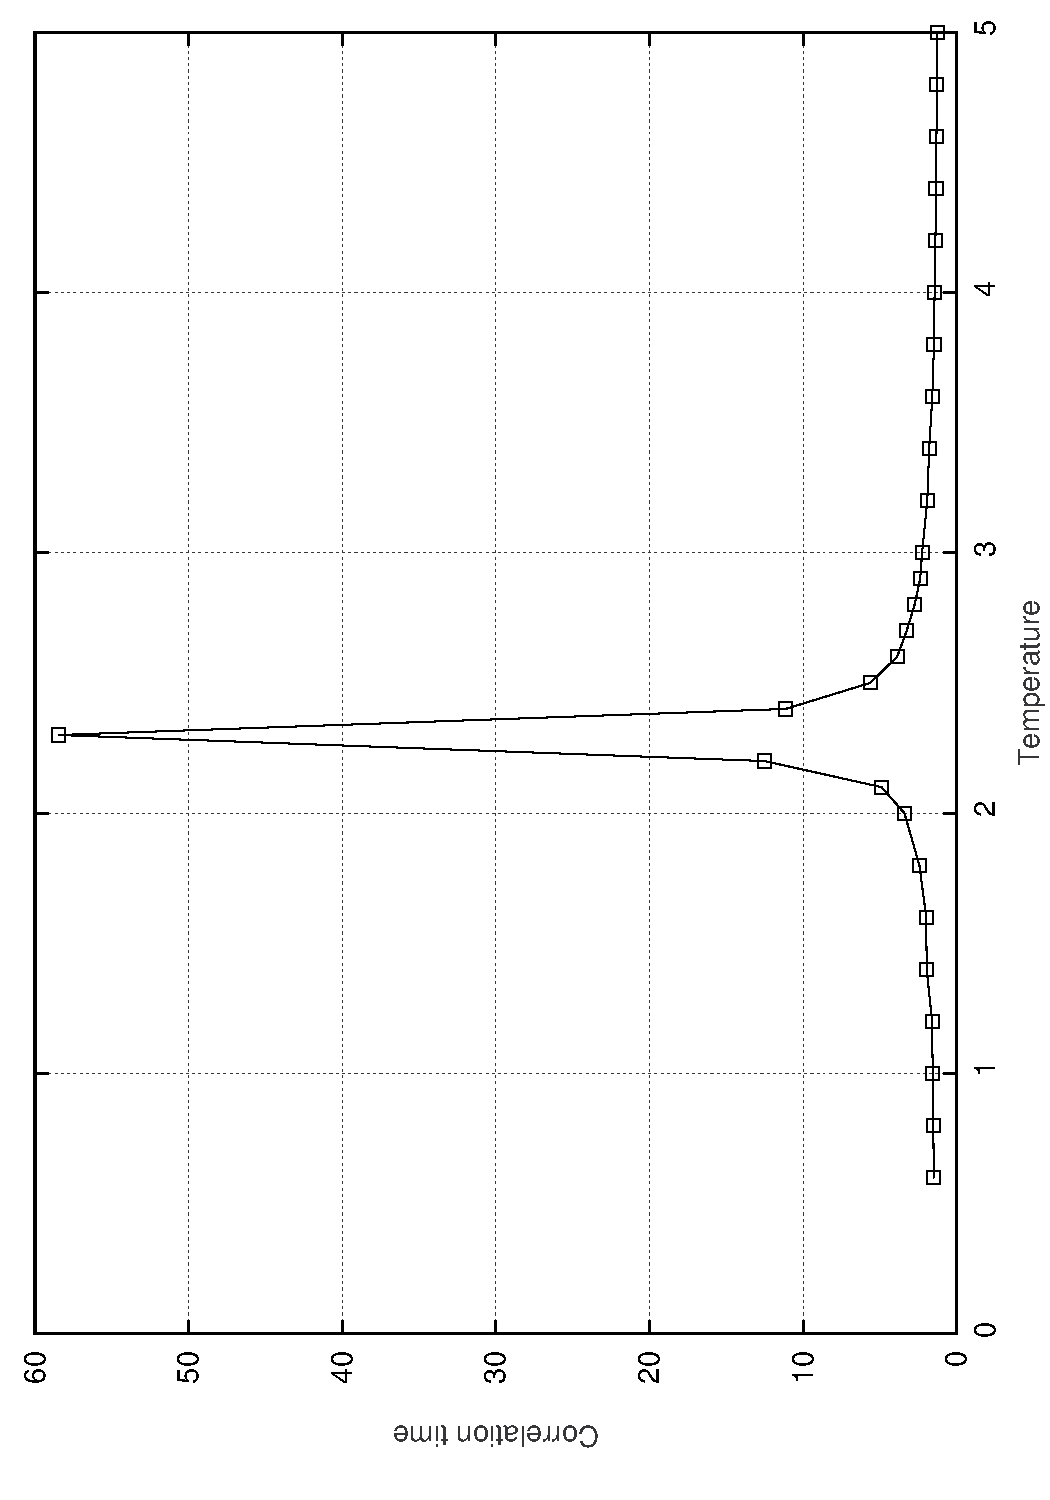
\includegraphics[angle=270, width=0.4\textwidth]{images/ctimes}
	\caption{{\footnotesize Gráfico de $\tau(T')$ para o modelo de Ising, onde T' é a temperatura reduzida ($T'\equiv\frac{k_b T}{J}$), com os pontos experimentais ligados por uma linha. A estimativa do tempo foi obtida após equilibrar o sistema (rede com L = 100) com 10000 MCS (passos de monte carlo), calculando a função de autocorrelação (eq.7) e integrando-a, assumindo a forma exponencial já referida.}}
	\label{fig:1}
\end{figurehere}
\end{multicols}

\begin{table}[h!]
\centering
\begin{tabular}{c c}
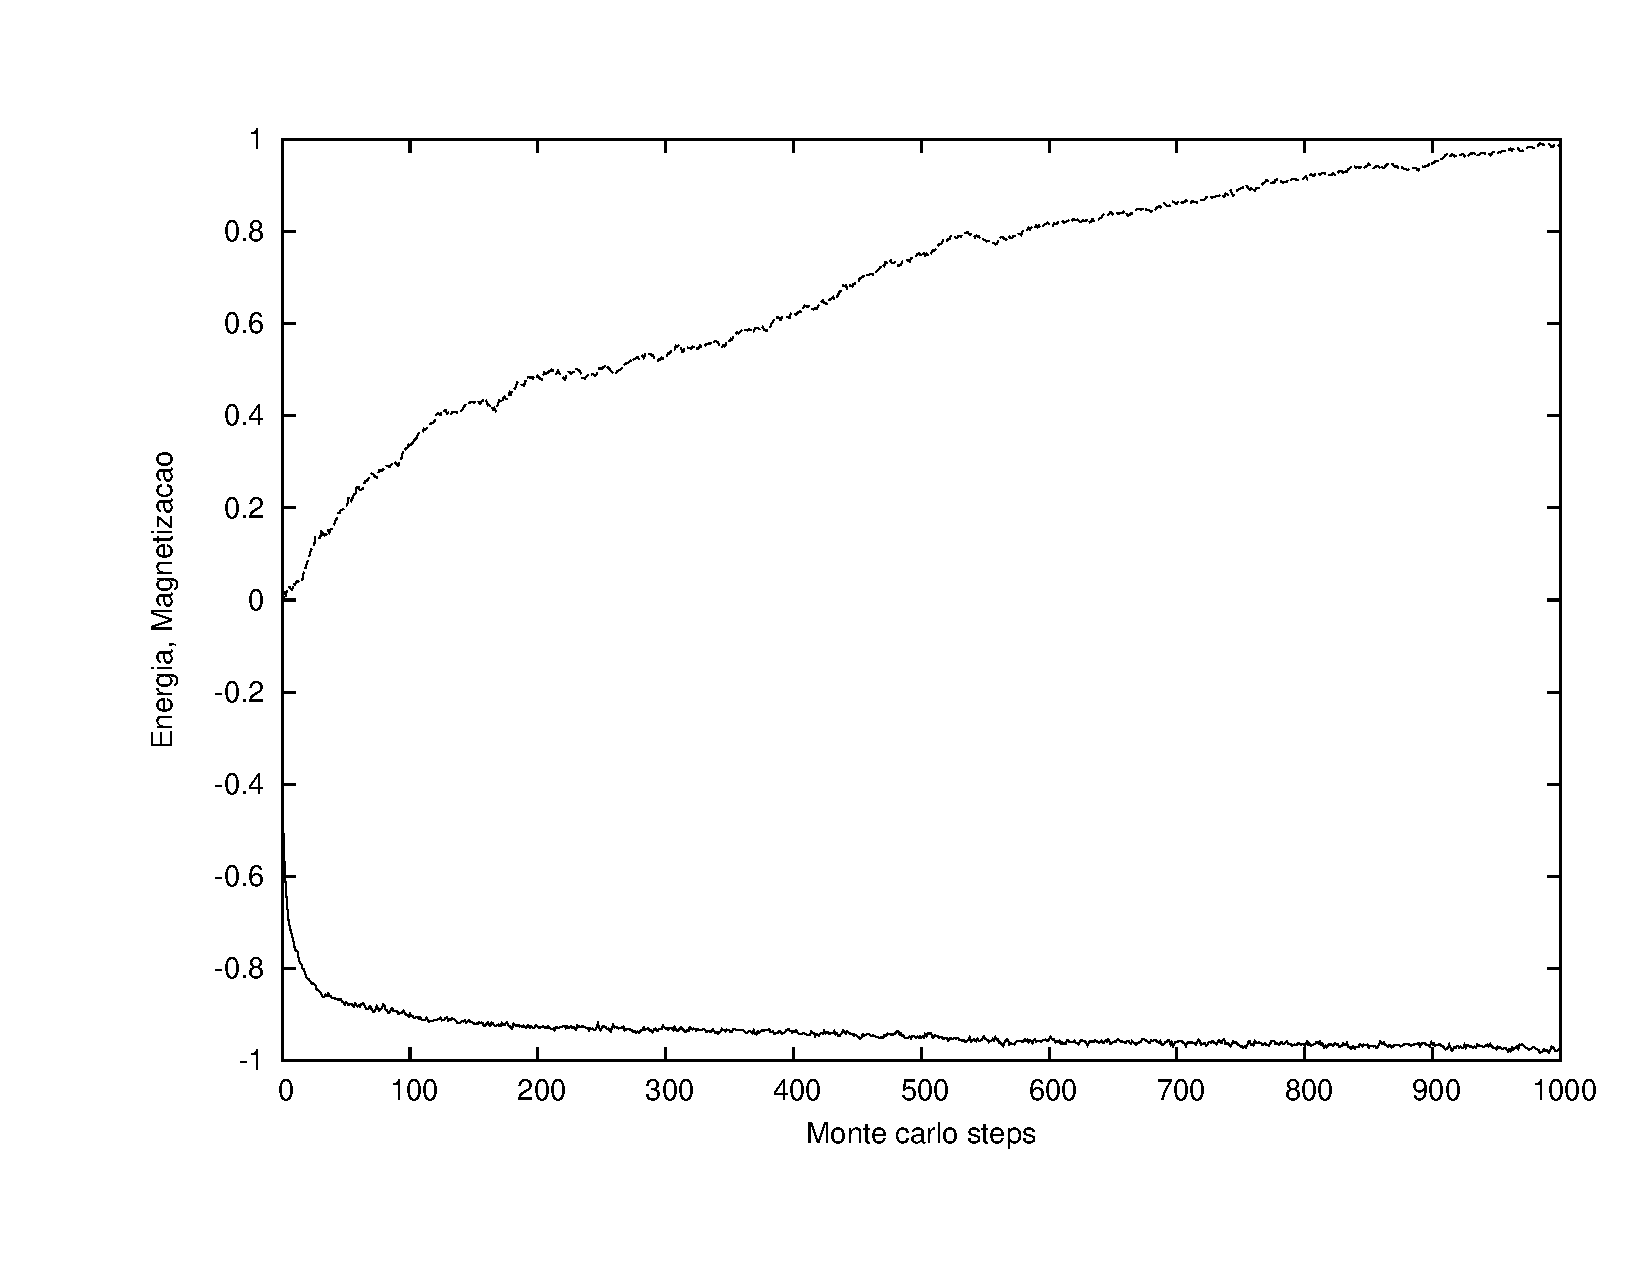
\includegraphics[angle=0, width=0.5\textwidth]{images/vars15}&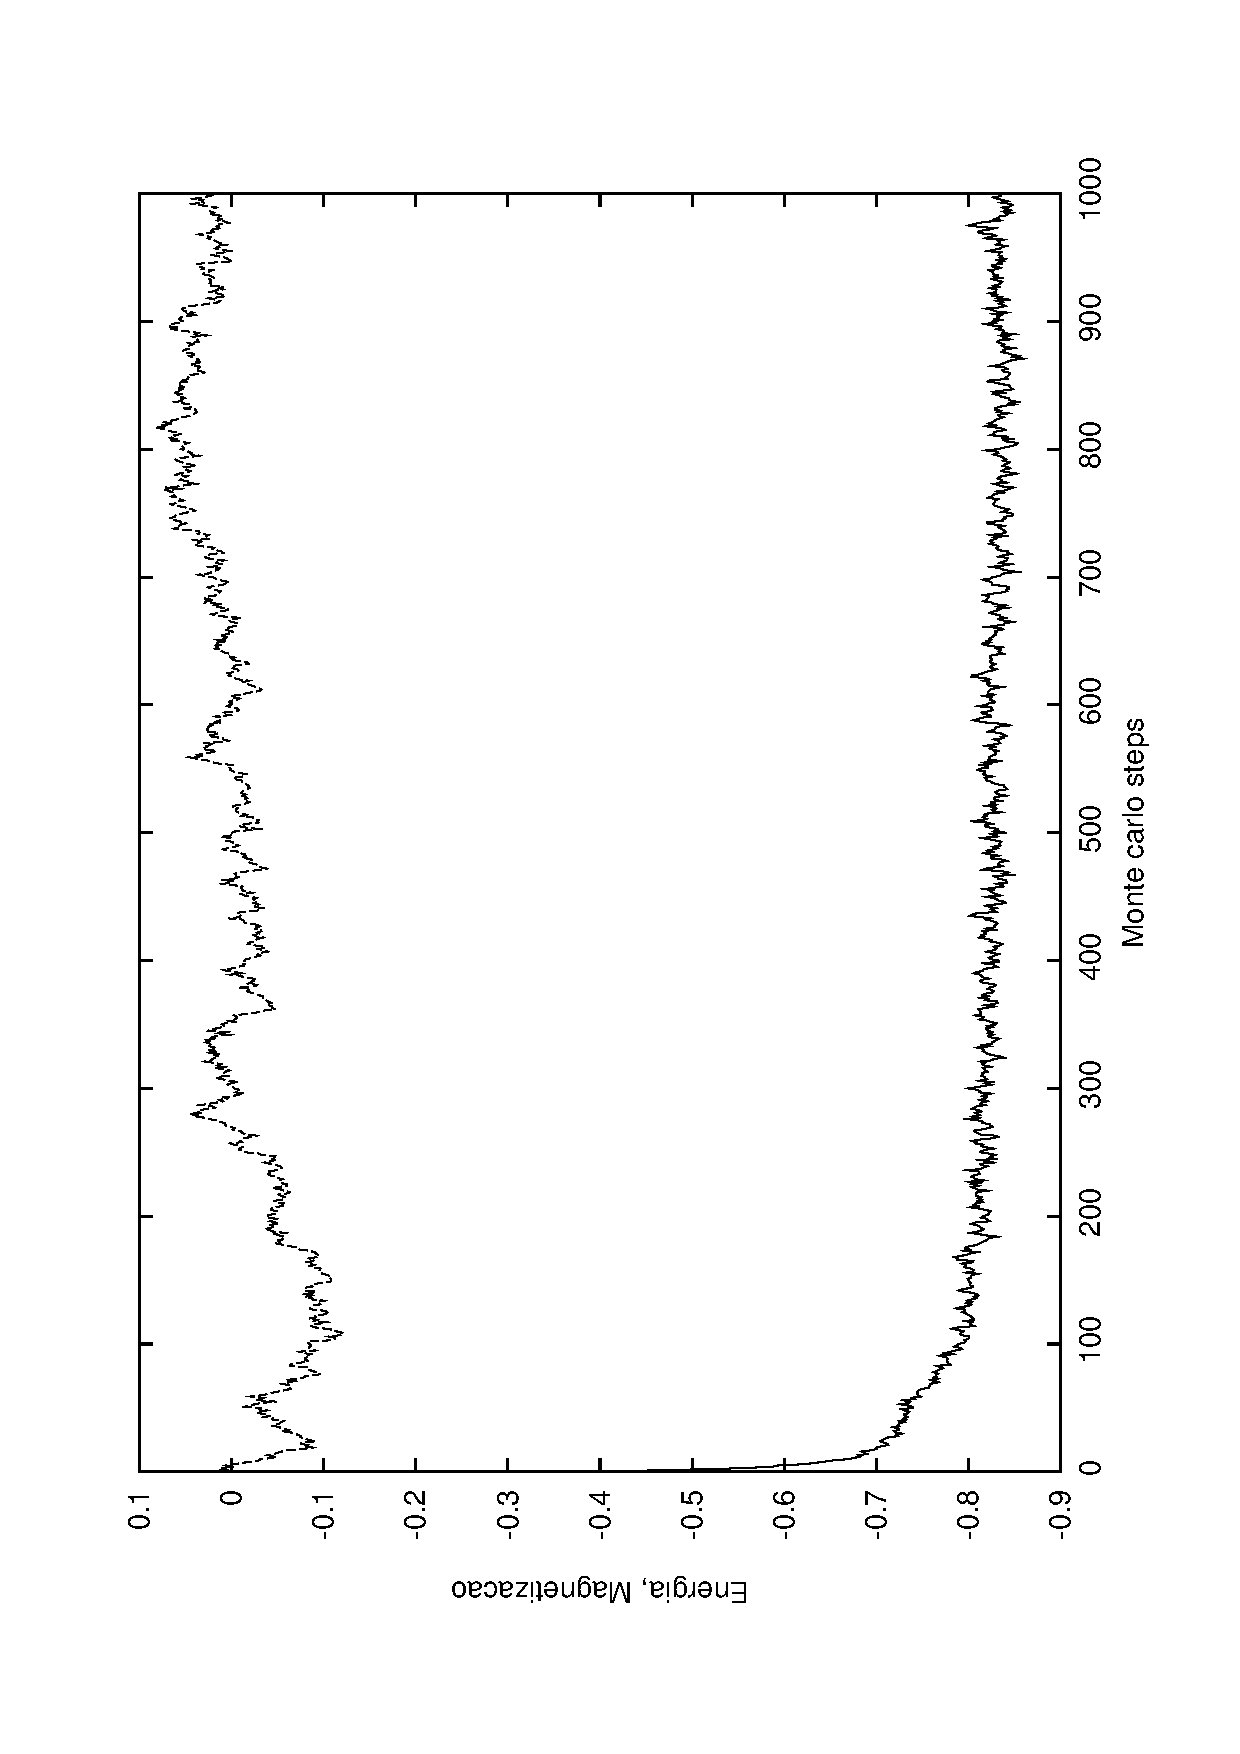
\includegraphics[angle=0, width=0.5\textwidth]{images/vars2}\\
\newline
{\footnotesize T'=1.5}&{\footnotesize T'=2}\\
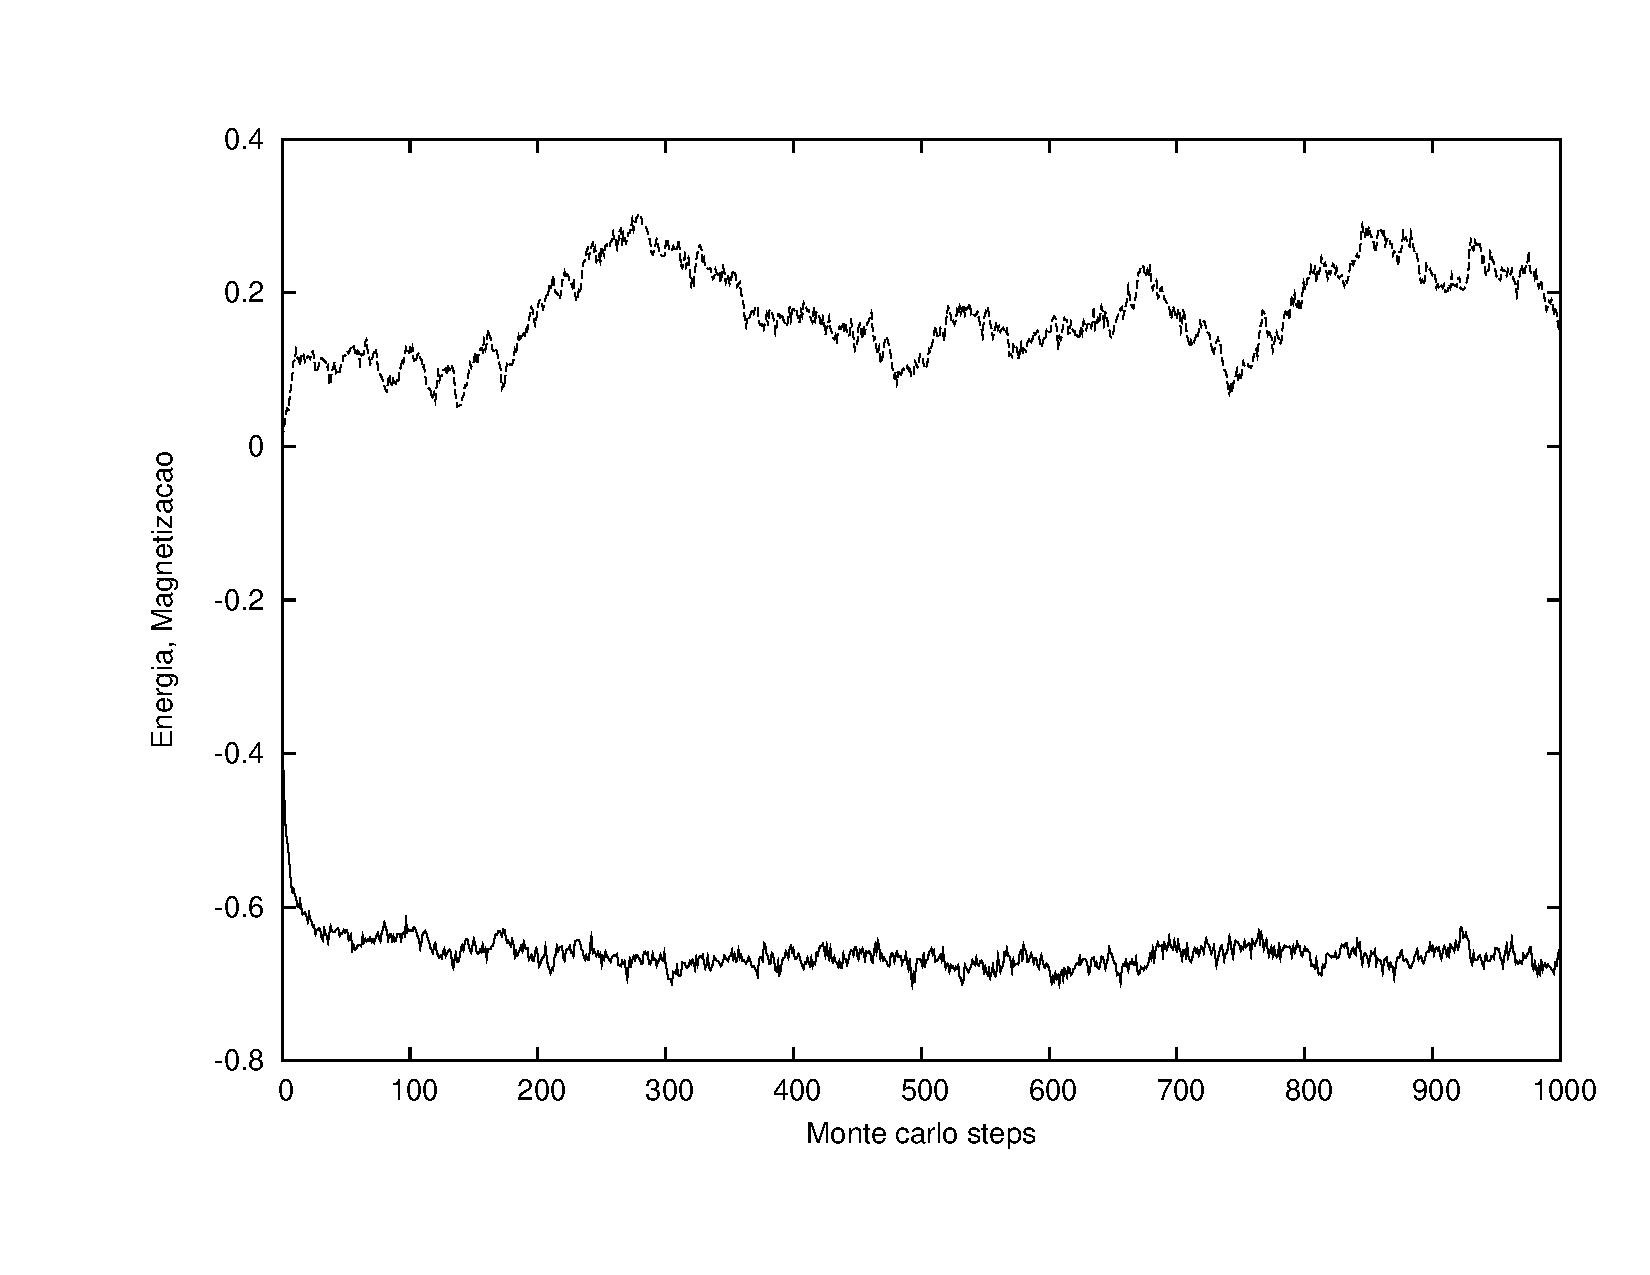
\includegraphics[angle=0, width=0.5\textwidth]{images/vars23}&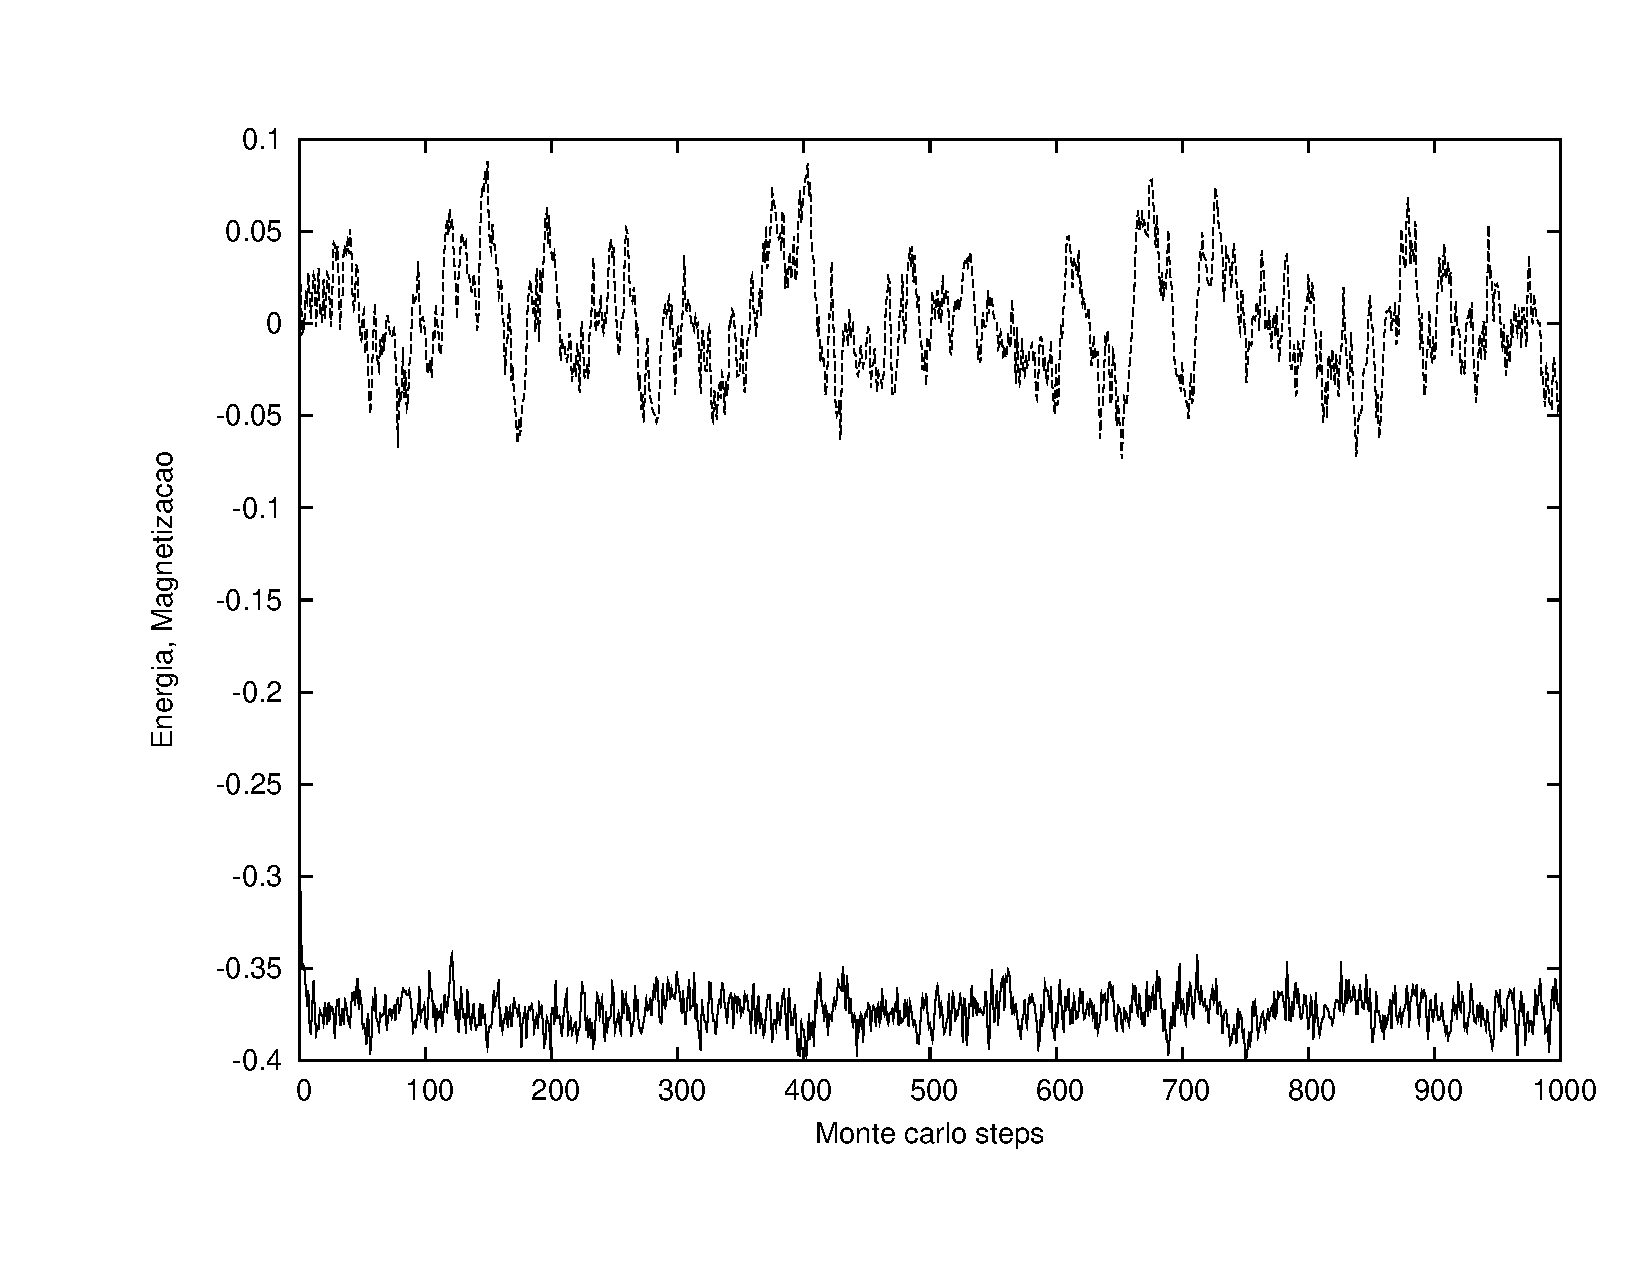
\includegraphics[angle=0, width=0.5\textwidth]{images/vars32}\\
{\footnotesize T'=2.3 ($\simeq T_c$)}&{\footnotesize T'=3.2}
\end{tabular}
\caption{Evolução da energia e magnetização para várias temperaturas. Os gráficos demonstram o sistema (rede com L = 100) a evoluir para o equilíbrio, minimizando a energia. As quantidades apresentadas são novamente reduzidas, com $m =\frac{M}{N}$ onde $M=\sum_i s_i$ e $E'=\frac{E}{2N}$. }
 \label{tab:1}
\end{table}

\begin{multicols}{2}

\subsection{Modelo de Agregação linear a 2D}

\subsubsection{Visualização}

\begin{figurehere}
	\centering
		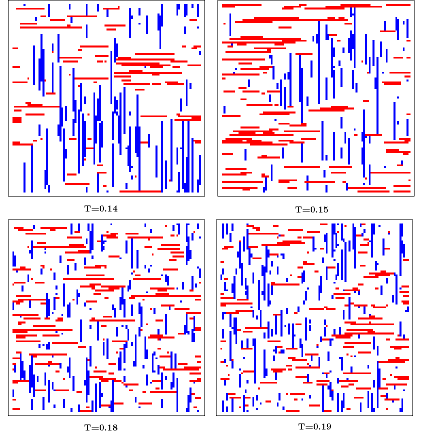
\includegraphics[width=0.5\textwidth]{images/rods2d}
	\caption{{\footnotesize Visualização do sistema 2D para $T' = \lbrace 0.14, 0.15 \; ( \simeq T_c ), 0.18, 1.9\rbrace$, onde as partículas são representadas por quadrados vermelhos e azuis, respectivamente horizontais e verticais.}}     
	\label{fig:2}
\end{figurehere}

\subsubsection{Resultados experimentais}

\begin{figurehere}
	\centering
		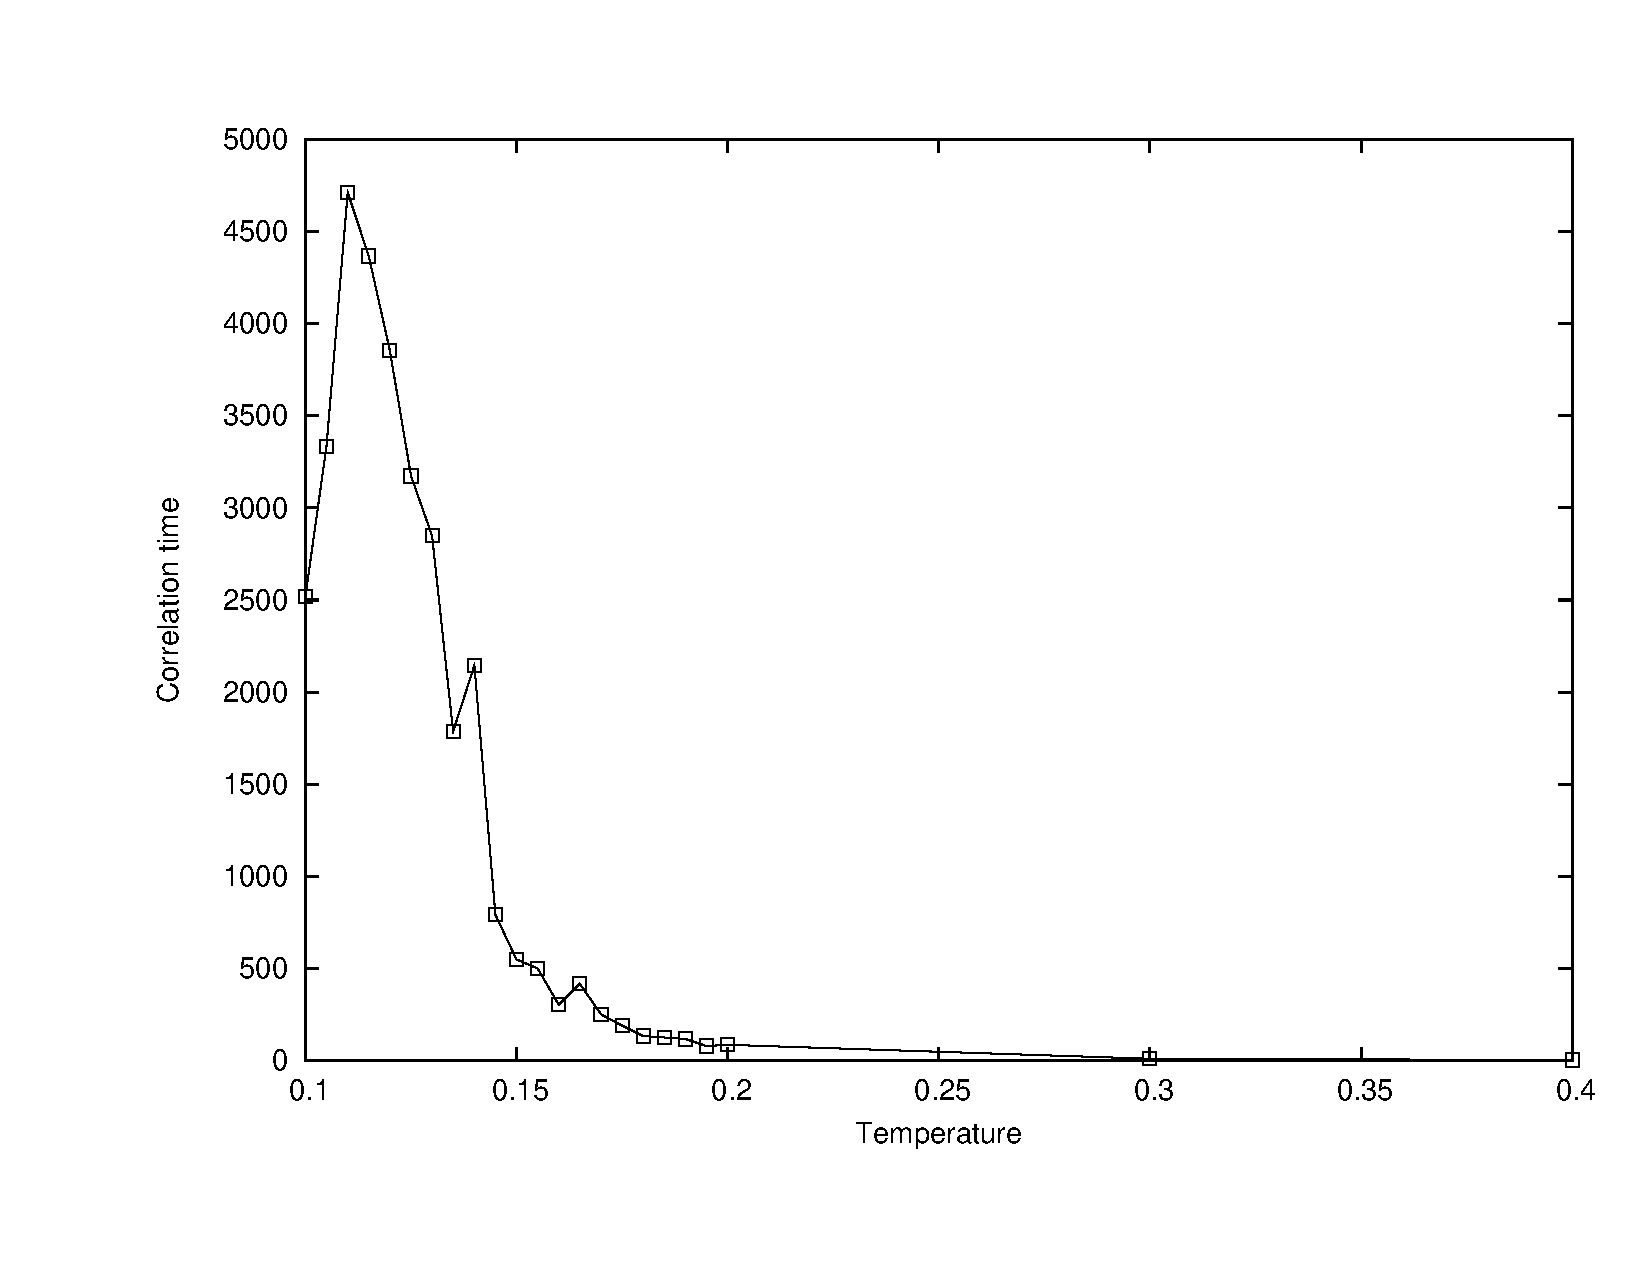
\includegraphics[width=0.5\textwidth]{images/ctimesr2d}
	\caption{{\footnotesize Gráfico de $\tau(T')$ para o modelo de agregação a 2D com $\rho = 0.2$, onde T' é a temperatura reduzida ($T'\equiv\frac{k_b T}{\epsilon}$), com os pontos experimentais ligados por uma linha. A estimativa do tempo foi obtida após equilibrar o sistema com 100000 MCS (passos de monte carlo), calculando a função de autocorrelação (eq.7) e integrando-a, assumindo a forma exponencial já referida.}}
	\label{fig:3}
\end{figurehere}

\begin{figurehere}
	\centering
		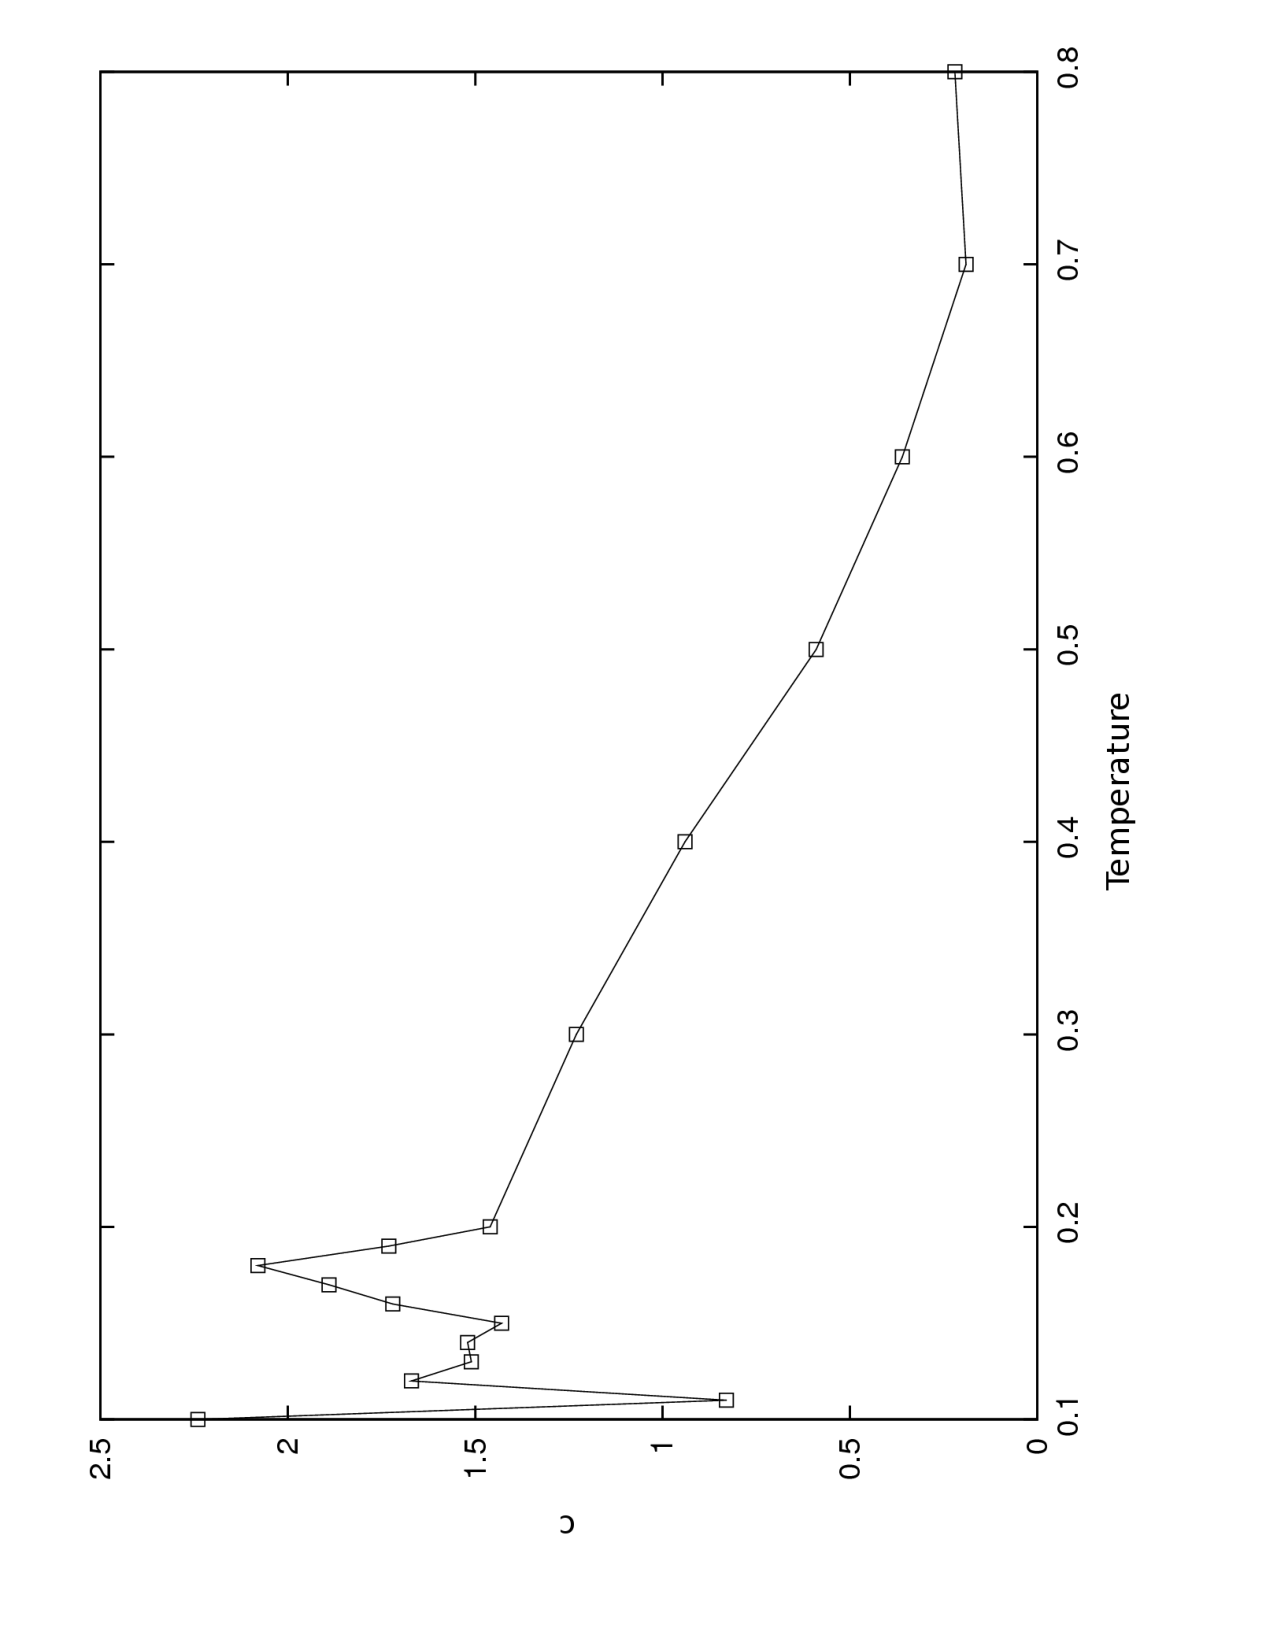
\includegraphics[angle=-90, width=0.5\textwidth]{images/c2d}
	\caption{{\footnotesize Calor específico $c$ para o modelo de agregação a 2D com $\rho = 0.2$, calculado após equilibrar o sistema esperando 100000 MCS e fazendo 20 medições da energia a cada 2 tempos de correlação, calculando então as suas flutuações.}}
	\label{fig:4}
\end{figurehere}

\begin{figurehere}
	\centering
		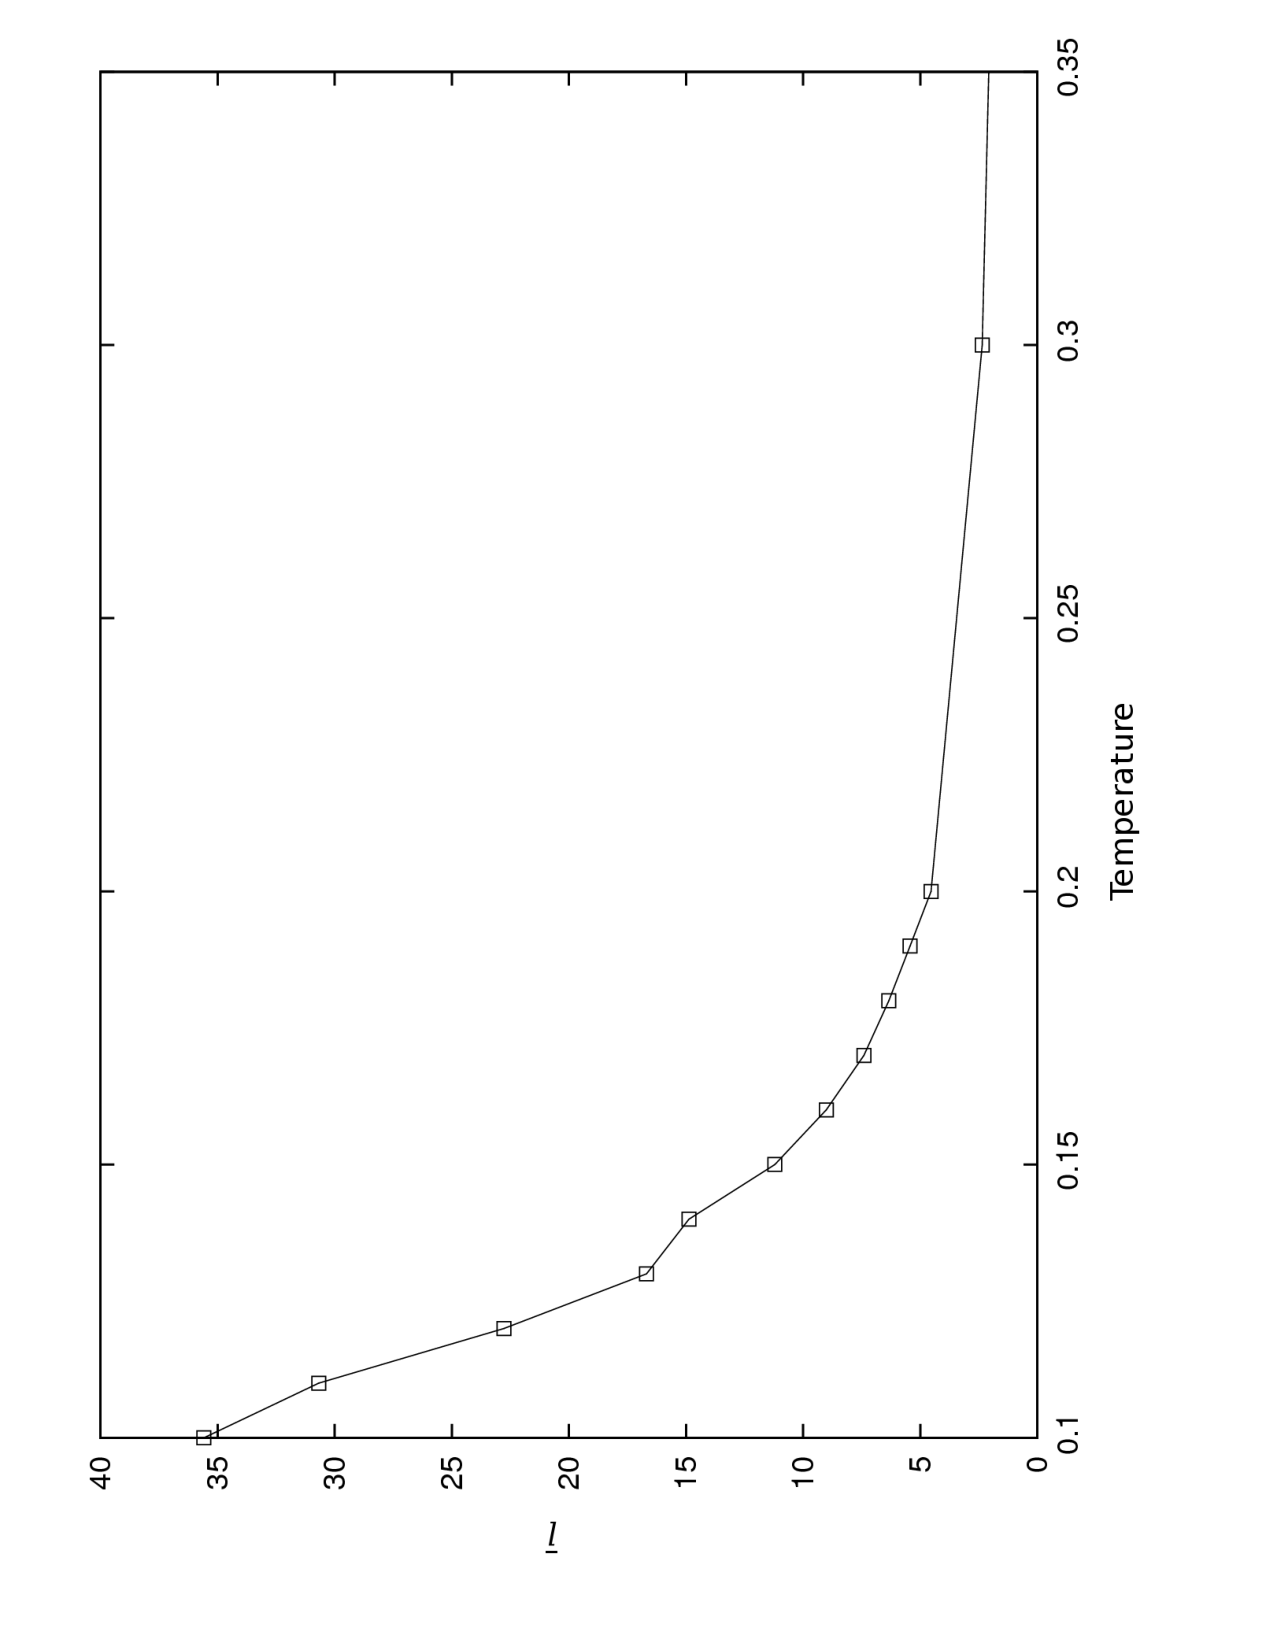
\includegraphics[angle=-90, width=0.5\textwidth]{images/lav2d}
	\caption{{\footnotesize Comprimento médio das cadeias $\bar{l}$ para o modelo de agregação a 2D com $\rho = 0.2$, calculado após equilibrar o sistema esperando 100000 MCS e fazendo 20 medições de $\bar{l}$ a cada 2 tempos de correlação, calculando então a sua média.}}
	\label{fig:5}
\end{figurehere}

\begin{figurehere}
	\centering
		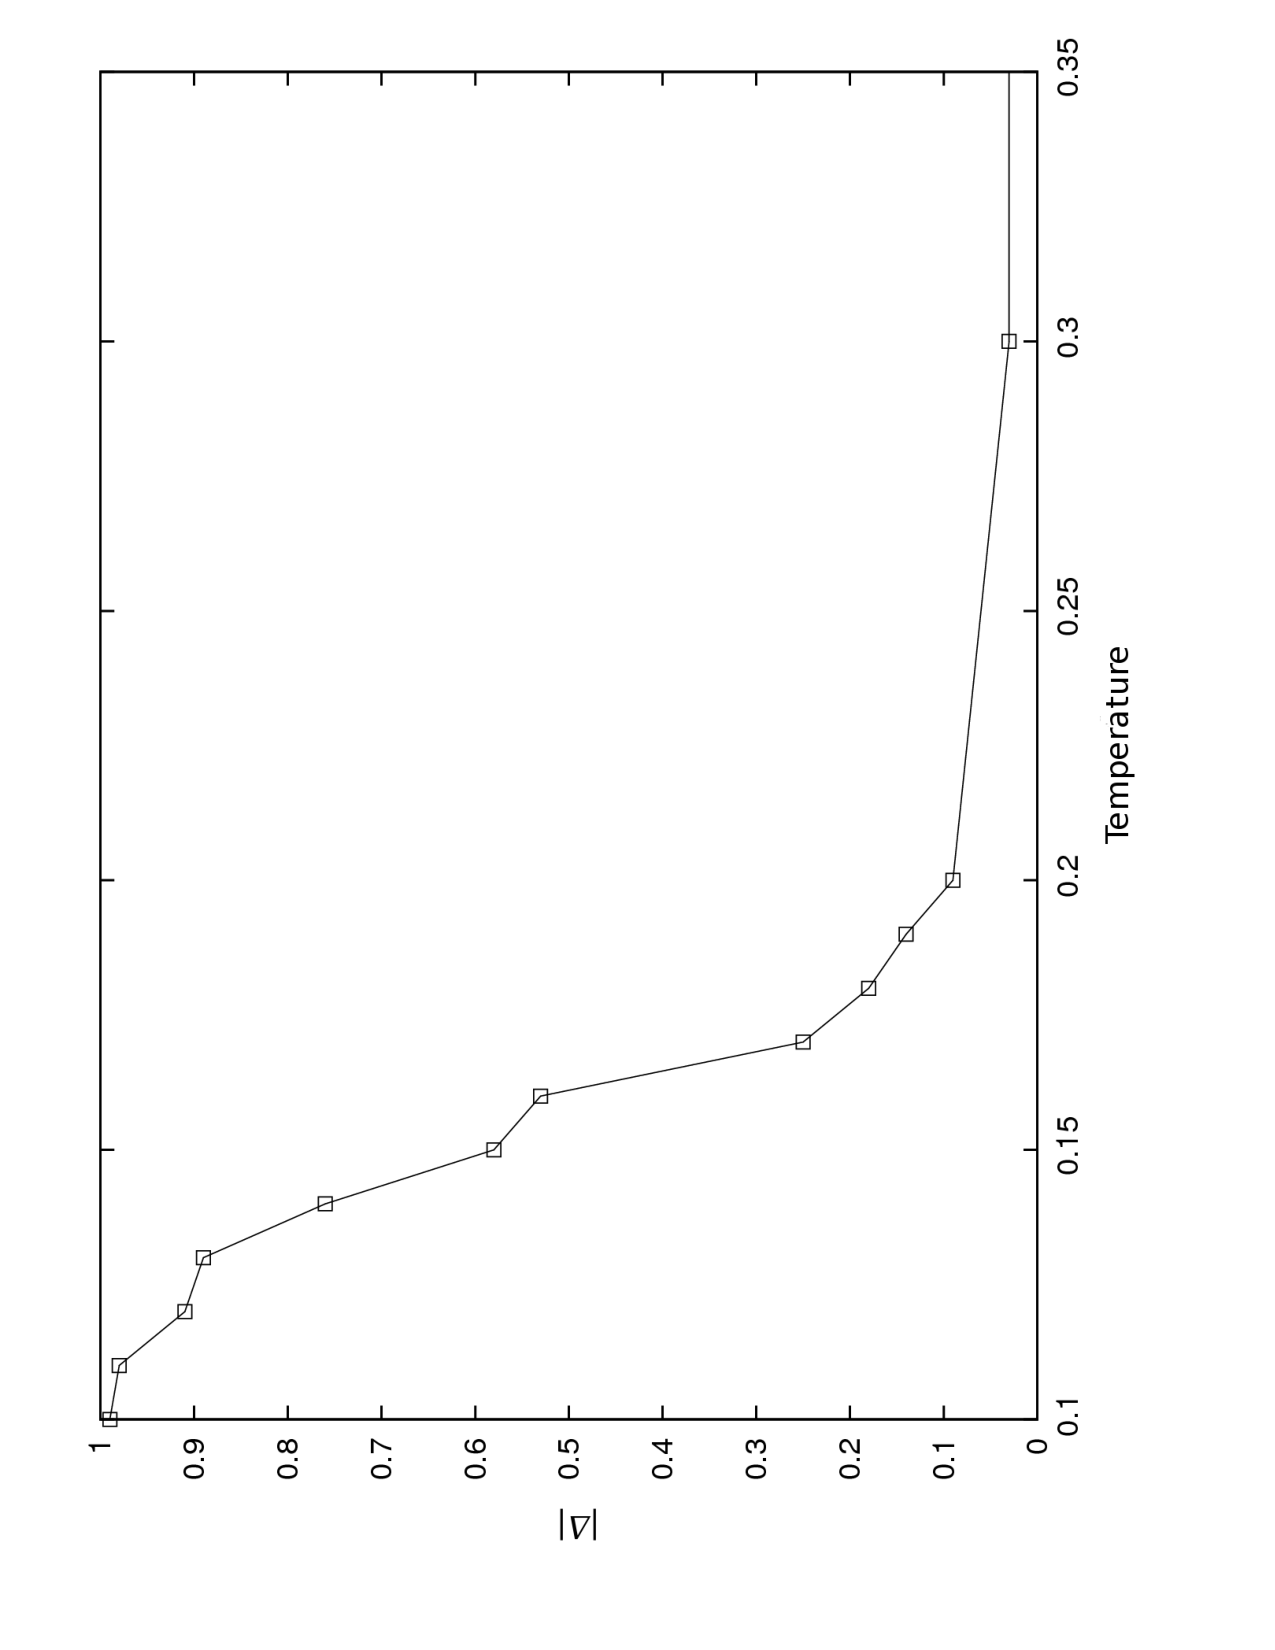
\includegraphics[angle=-90, width=0.5\textwidth]{images/delta2d}
	\caption{{\footnotesize Parâmetro de ordem reduzido $|\Delta|$ para o modelo de agregação a 2D com $\rho = 0.2$. O parâmetro foi calculado após equilibrar o sistema esperando 100000 MCS e fazendo 20 medições de $|\Delta|$ a cada 2 tempos de correlação, calculando então a sua média.}}
	\label{fig:6}
\end{figurehere}

\subsection{Modelo de Agregação linear a 3D}
\subsubsection{Resultados experimentais: $\rho=0.1$}

\begin{figurehere}
	\centering
		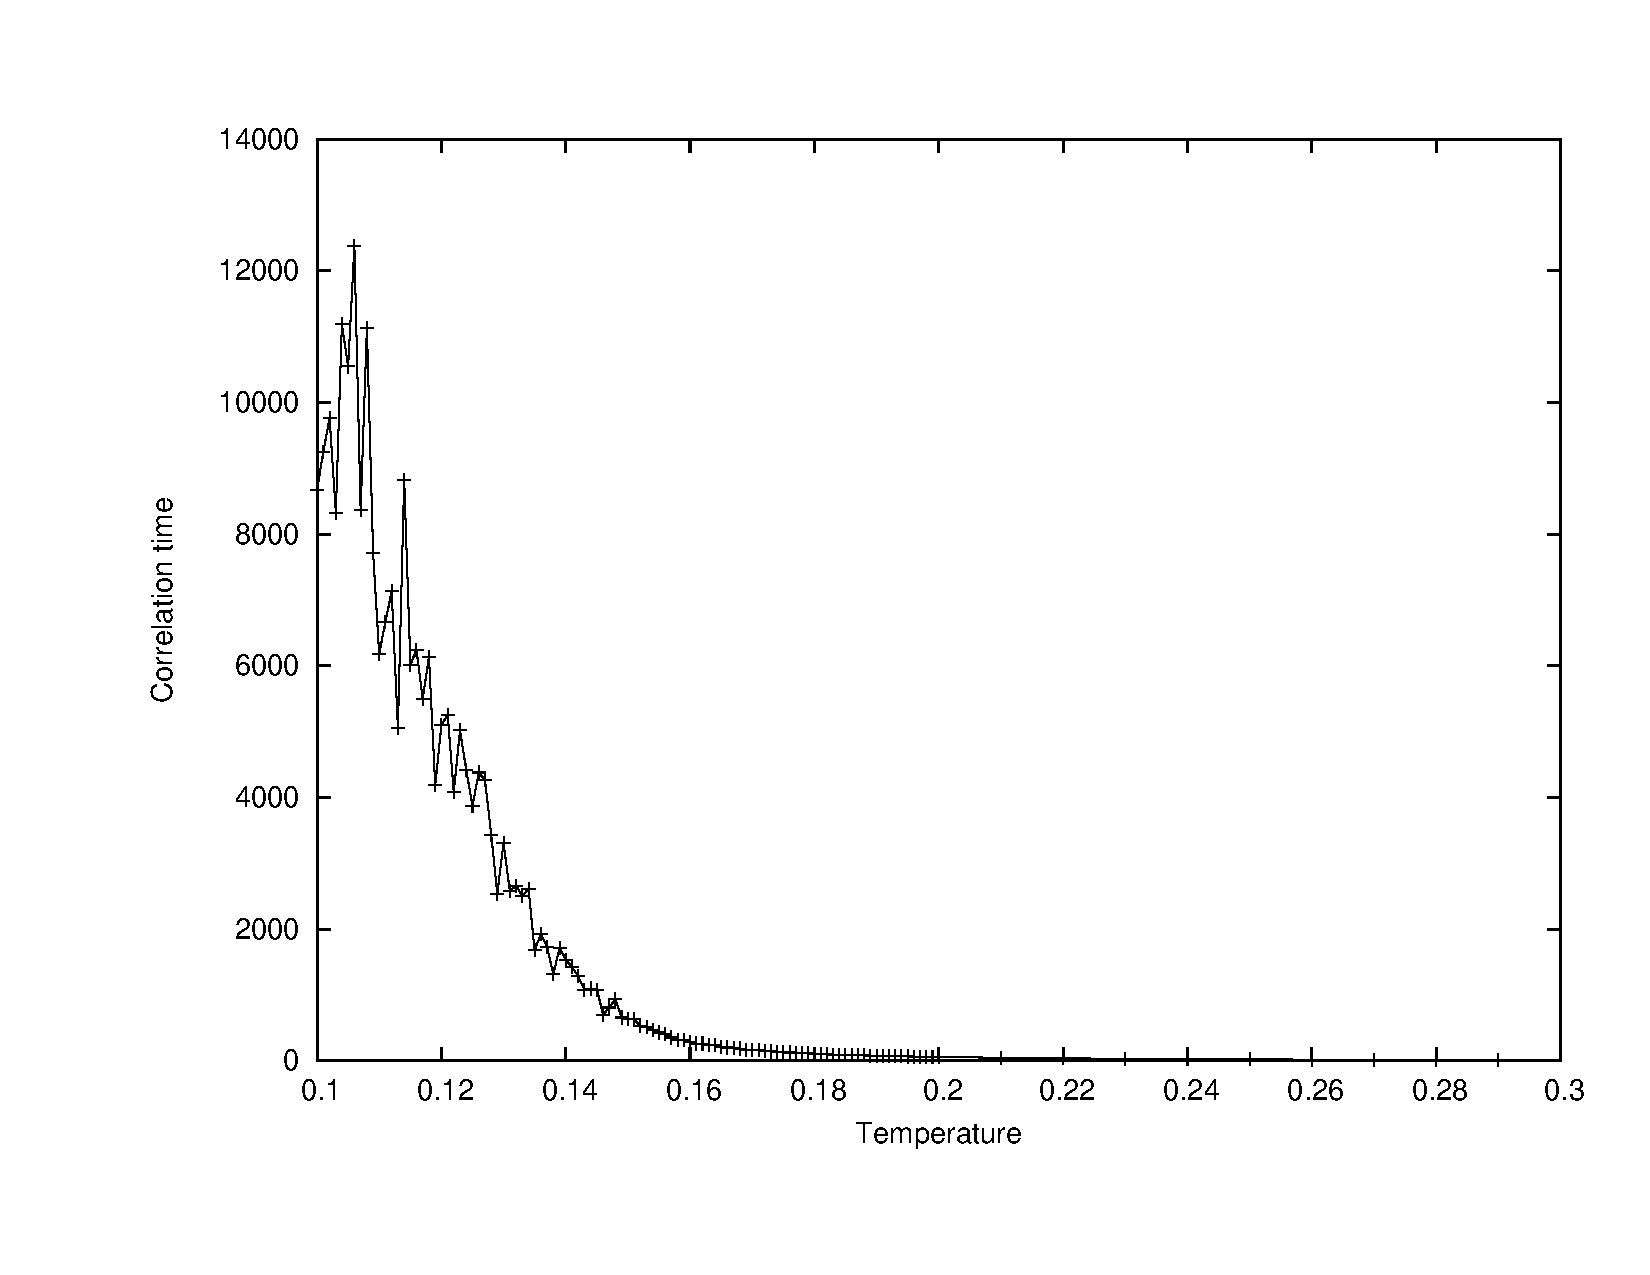
\includegraphics[width=0.5\textwidth, clip, trim = 1.7cm 1.5cm 1cm 1cm]{images/ctimes1}
	\caption{{\footnotesize Gráfico de $\tau(T')$ para o modelo de agregação a 3D, onde T' é a temperatura reduzida ($T'\equiv\frac{k_b T}{\varepsilon}$), para $\rho = 0.1$, com os pontos experimentais ligados por uma linha. A estimativa do tempo foi obtida após equilibrar o sistema com 500000 MCS (passos de monte carlo), calculando a função de autocorrelação (eq.7) e integrando-a, assumindo a forma exponencial já referida.}}
	\label{fig:7}
\end{figurehere}

\begin{figurehere}
	\centering
		\includegraphics[width=0.5\textwidth, clip, trim = 1.7cm 1.5cm 1cm 1cm]{images/0.1/c}
	\caption{{\footnotesize Calor específico $c$ para $\rho = 0.1$, calculado após equilibrar o sistema esperando 500000 MCS e fazendo 20 medições da energia a cada 2 tempos de correlação, calculando então as suas flutuações.}}
	\label{fig:8}
\end{figurehere}

\begin{figurehere}
	\centering
		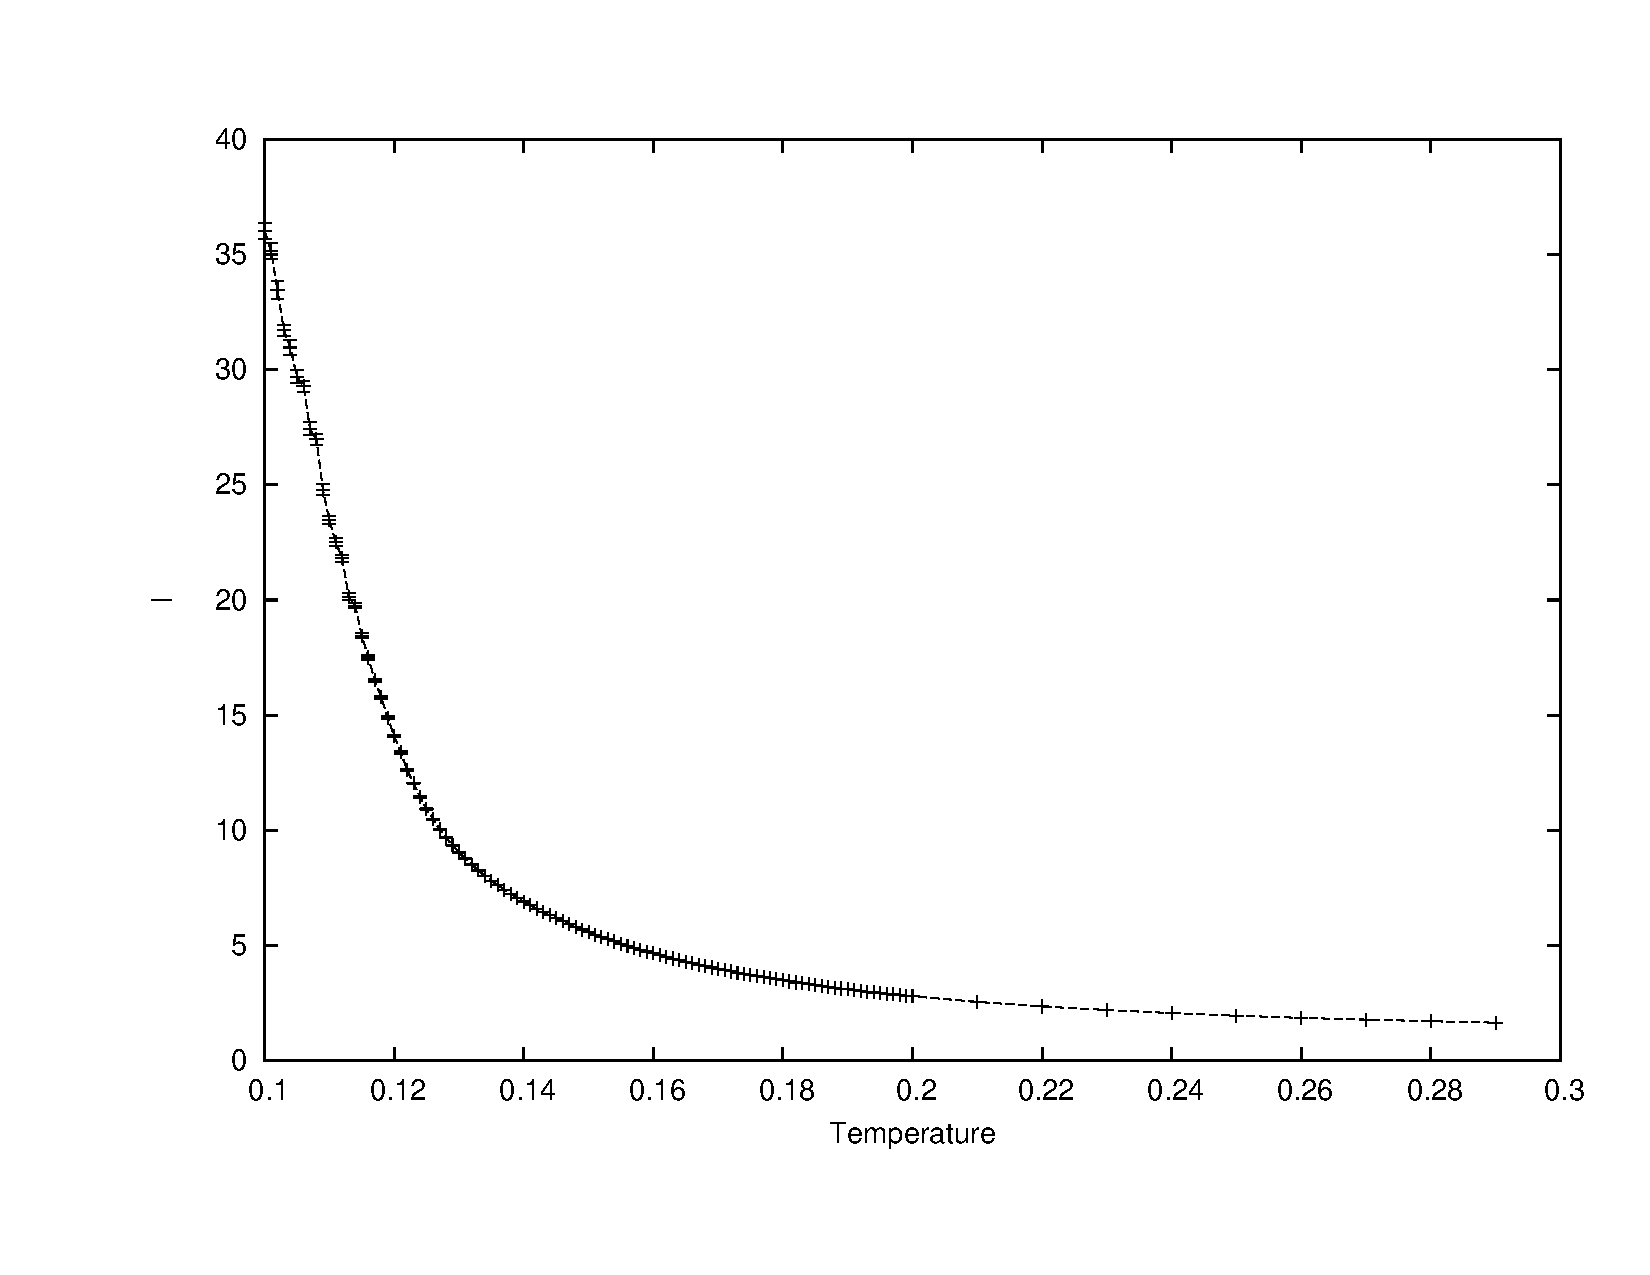
\includegraphics[width=0.5\textwidth, clip, trim = 1.7cm 1.5cm 1cm 1cm]{images/0.1/l}
	\caption{{\footnotesize Comprimento médio das cadeias $\bar{l}$ para $\rho = 0.1$, calculado após equilibrar o sistema esperando 500000 MCS e fazendo 20 medições de $\bar{l}$ a cada 2 tempos de correlação, calculando então a sua média.}}
	\label{fig:9}
\end{figurehere}

\begin{figurehere}
	\centering
		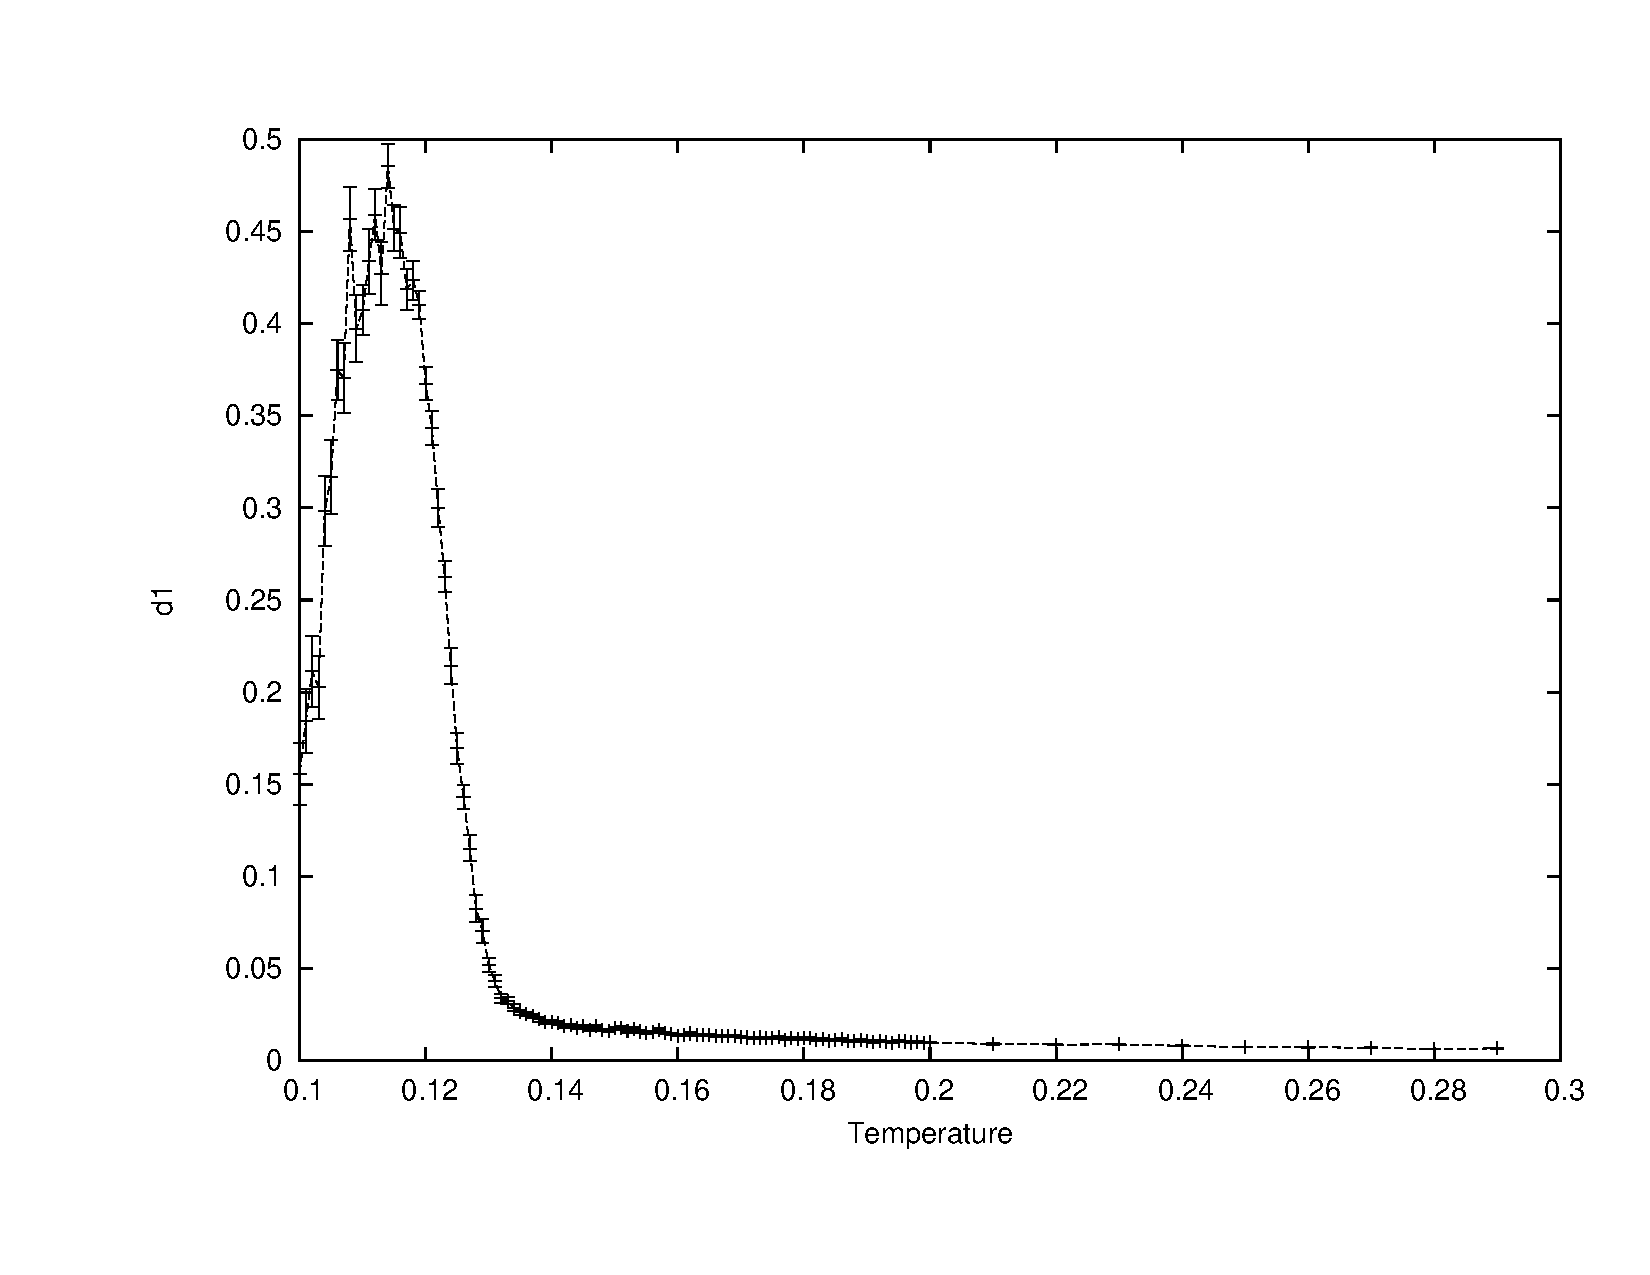
\includegraphics[width=0.5\textwidth, clip, trim = 1.7cm 1.5cm 1cm 1cm]{images/0.1/d1}
	\caption{{\footnotesize Parâmetro de ordem reduzido $|\Delta_1|$ para $\rho = 0.1$. O parâmetro foi calculado após equilibrar o sistema esperando 500000 MCS e fazendo 20 medições de $|\Delta_1|$ a cada 2 tempos de correlação, calculando então a sua média.}}
	\label{fig:10}
\end{figurehere}

\begin{figurehere}
	\centering
		\includegraphics[width=0.5\textwidth, clip, trim = 1.7cm 1.5cm 1cm 1cm]{images/0.1/d1f}
	\caption{{\footnotesize Flutuações do parâmetro de ordem reduzido $|\Delta_1|$ para $\rho = 0.1$, calculadas da mesma forma que c. Será em princípio possível ver a transição de fase determinando $T$ para a qual as flutuações tendem para infinito}}
	\label{fig:11}
\end{figurehere}

\begin{figurehere}
	\centering
		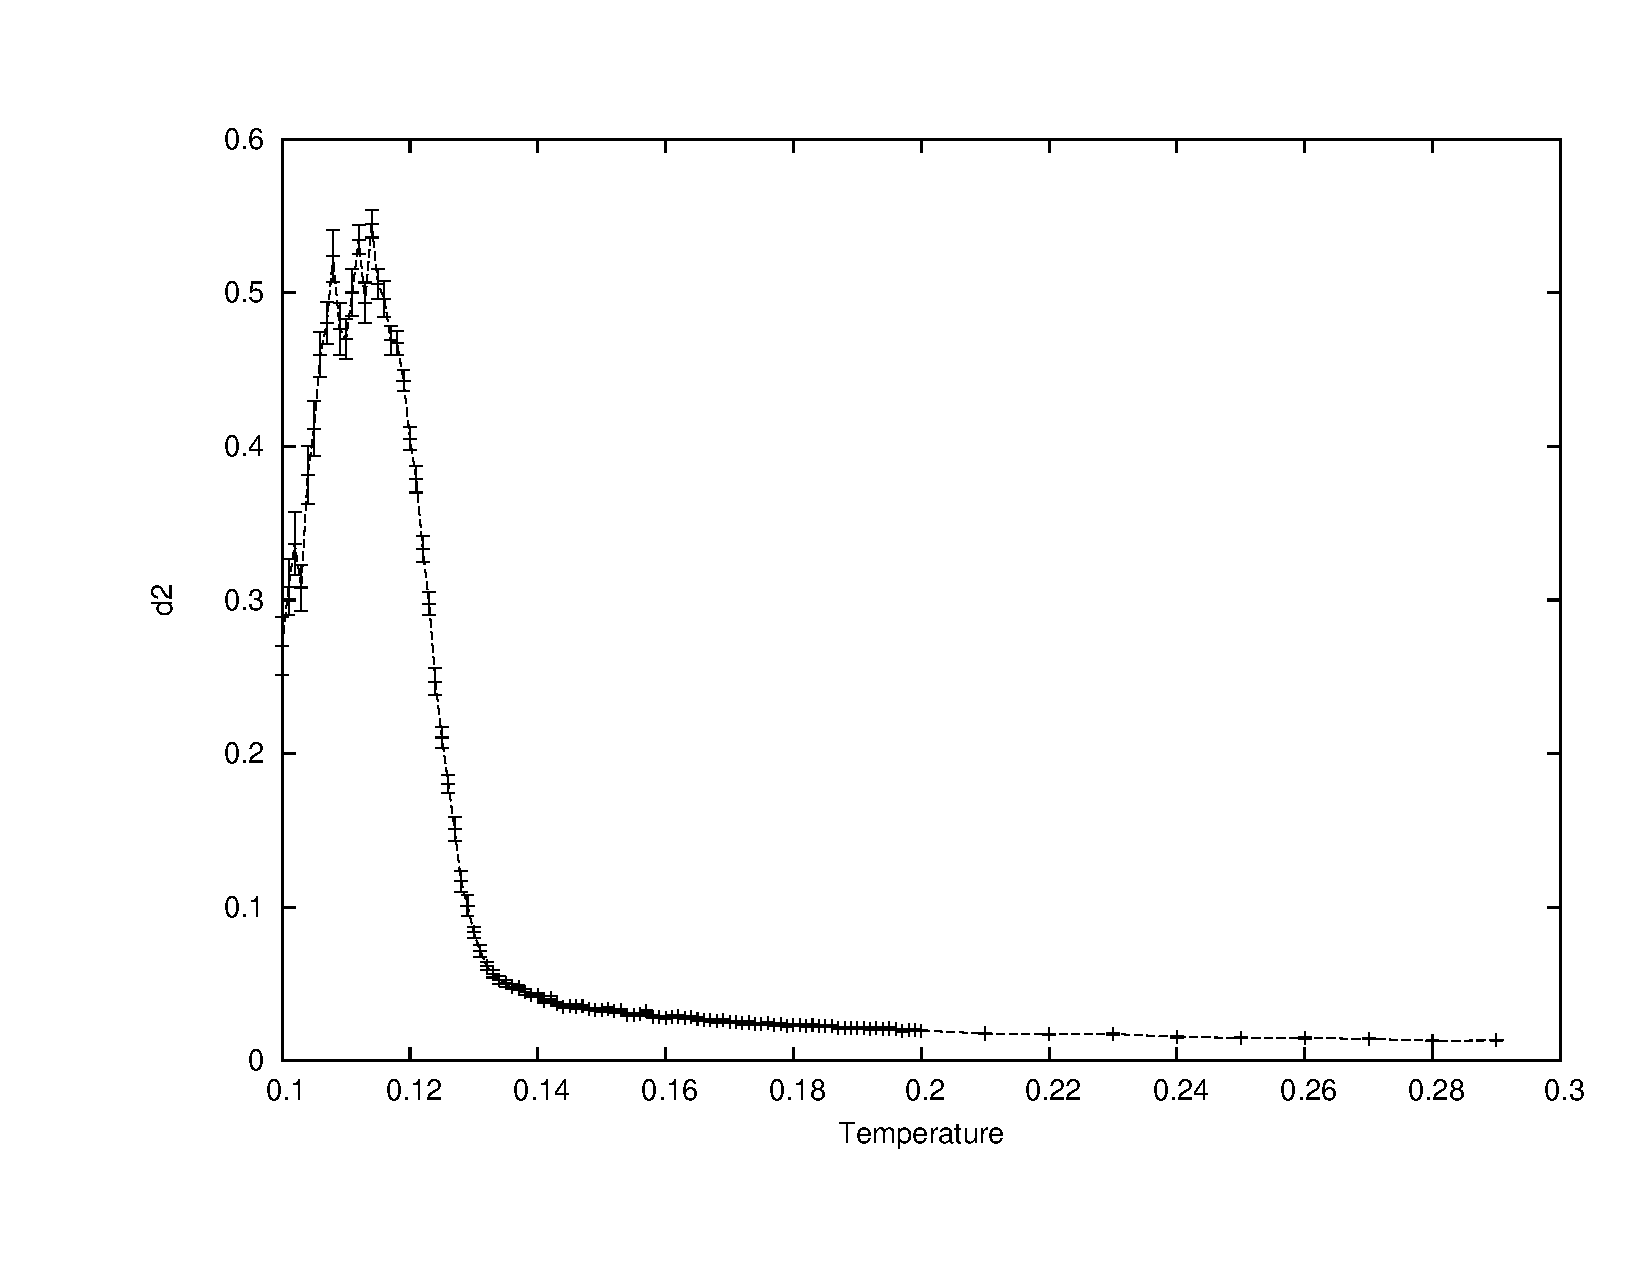
\includegraphics[width=0.5\textwidth, clip, trim = 1.7cm 1.5cm 1cm 1cm]{images/0.1/d2}
	\caption{{\footnotesize Parâmetro de ordem reduzido $|\Delta_2|$ para $\rho = 0.1$. O parâmetro foi calculado após equilibrar o sistema esperando 500000 MCS e fazendo 20 medições de $|\Delta_2|$ a cada 2 tempos de correlação, calculando então a sua média.}}
	\label{fig:12}
\end{figurehere}

\begin{figurehere}
	\centering
		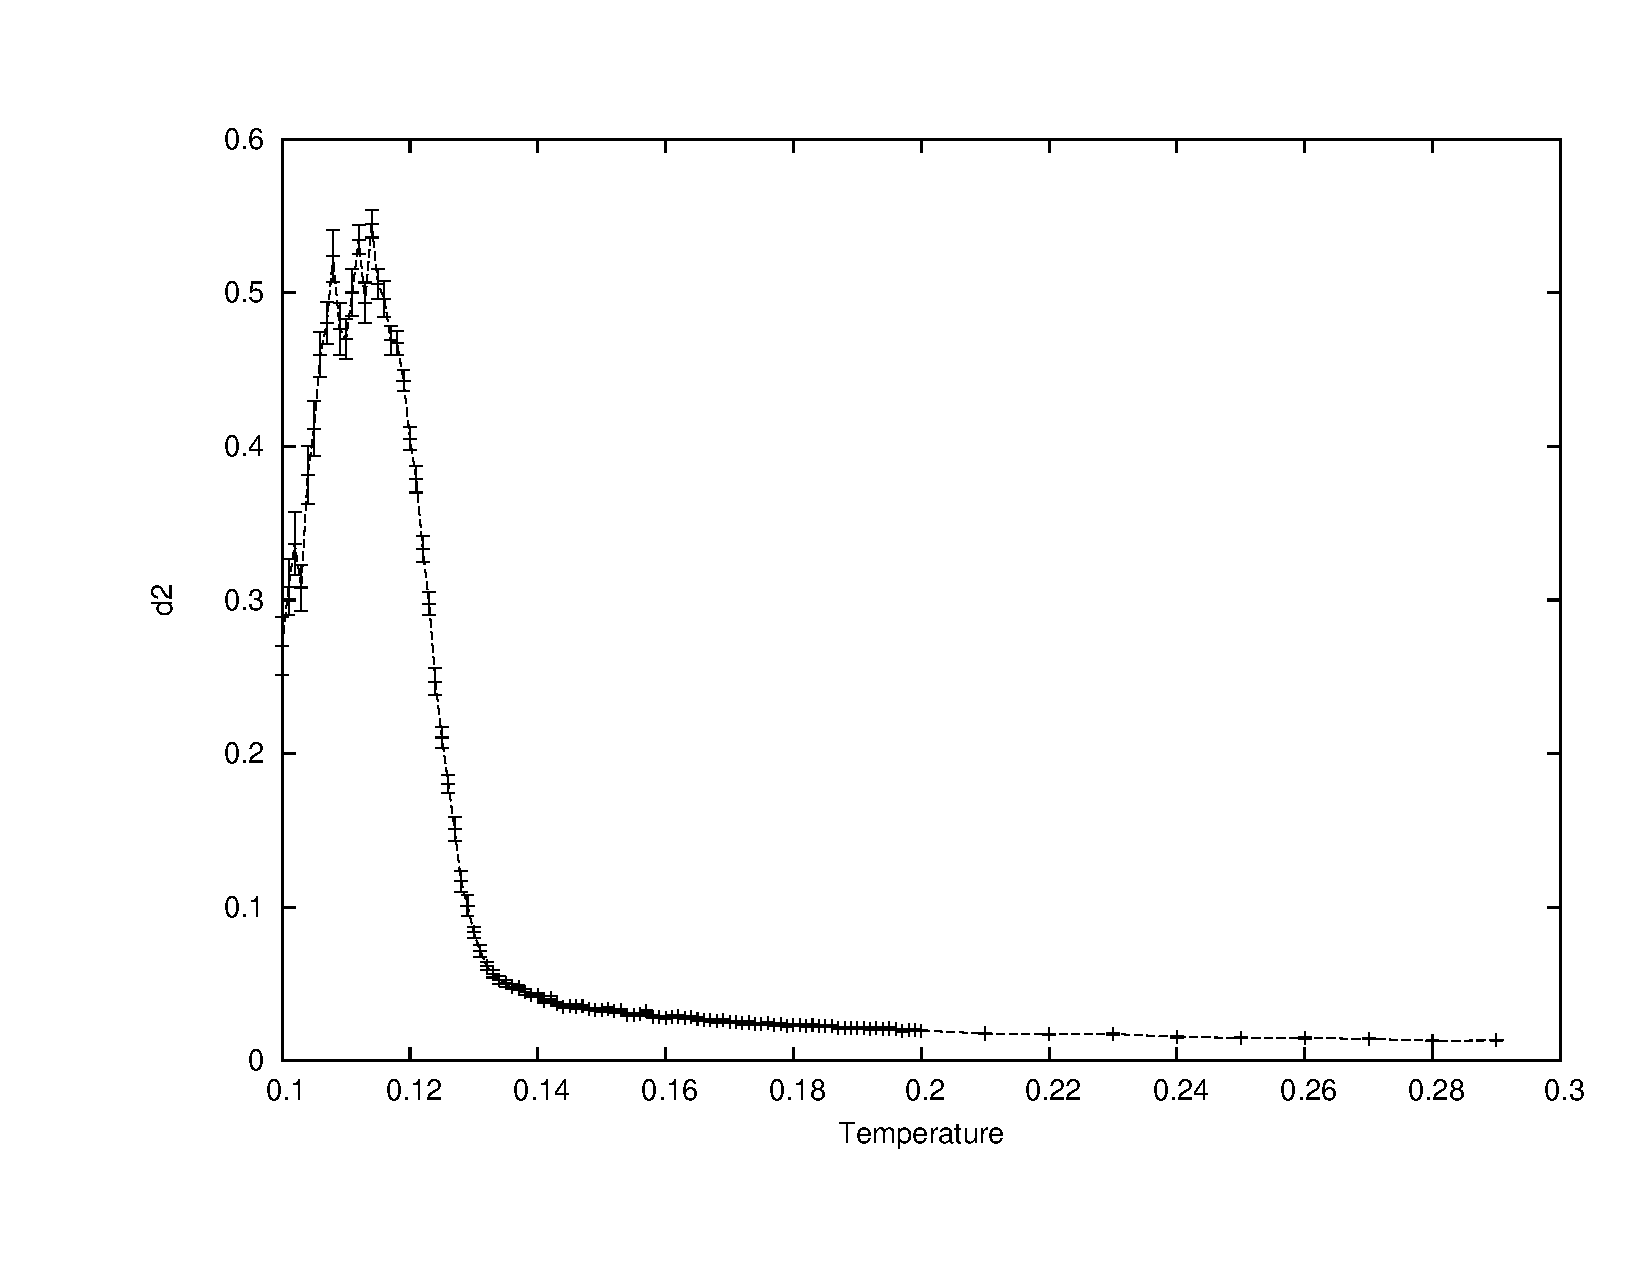
\includegraphics[width=0.5\textwidth, clip, trim = 1.7cm 1.5cm 1cm 1cm]{images/0.1/d2}
	\caption{{\footnotesize Flutuações do parâmetro de ordem reduzido $\frac{|\Delta_2|}{N}$ para $\rho = 0.1$, calculadas da mesma forma que c. Será em princípio possível ver a transição de fase determinando $T$ para a qual as flutuações tendem para infinito}}
	\label{fig:13}
\end{figurehere}

\subsubsection{Resultados experimentais: $\rho=0.2$}

\begin{figurehere}
	\centering
		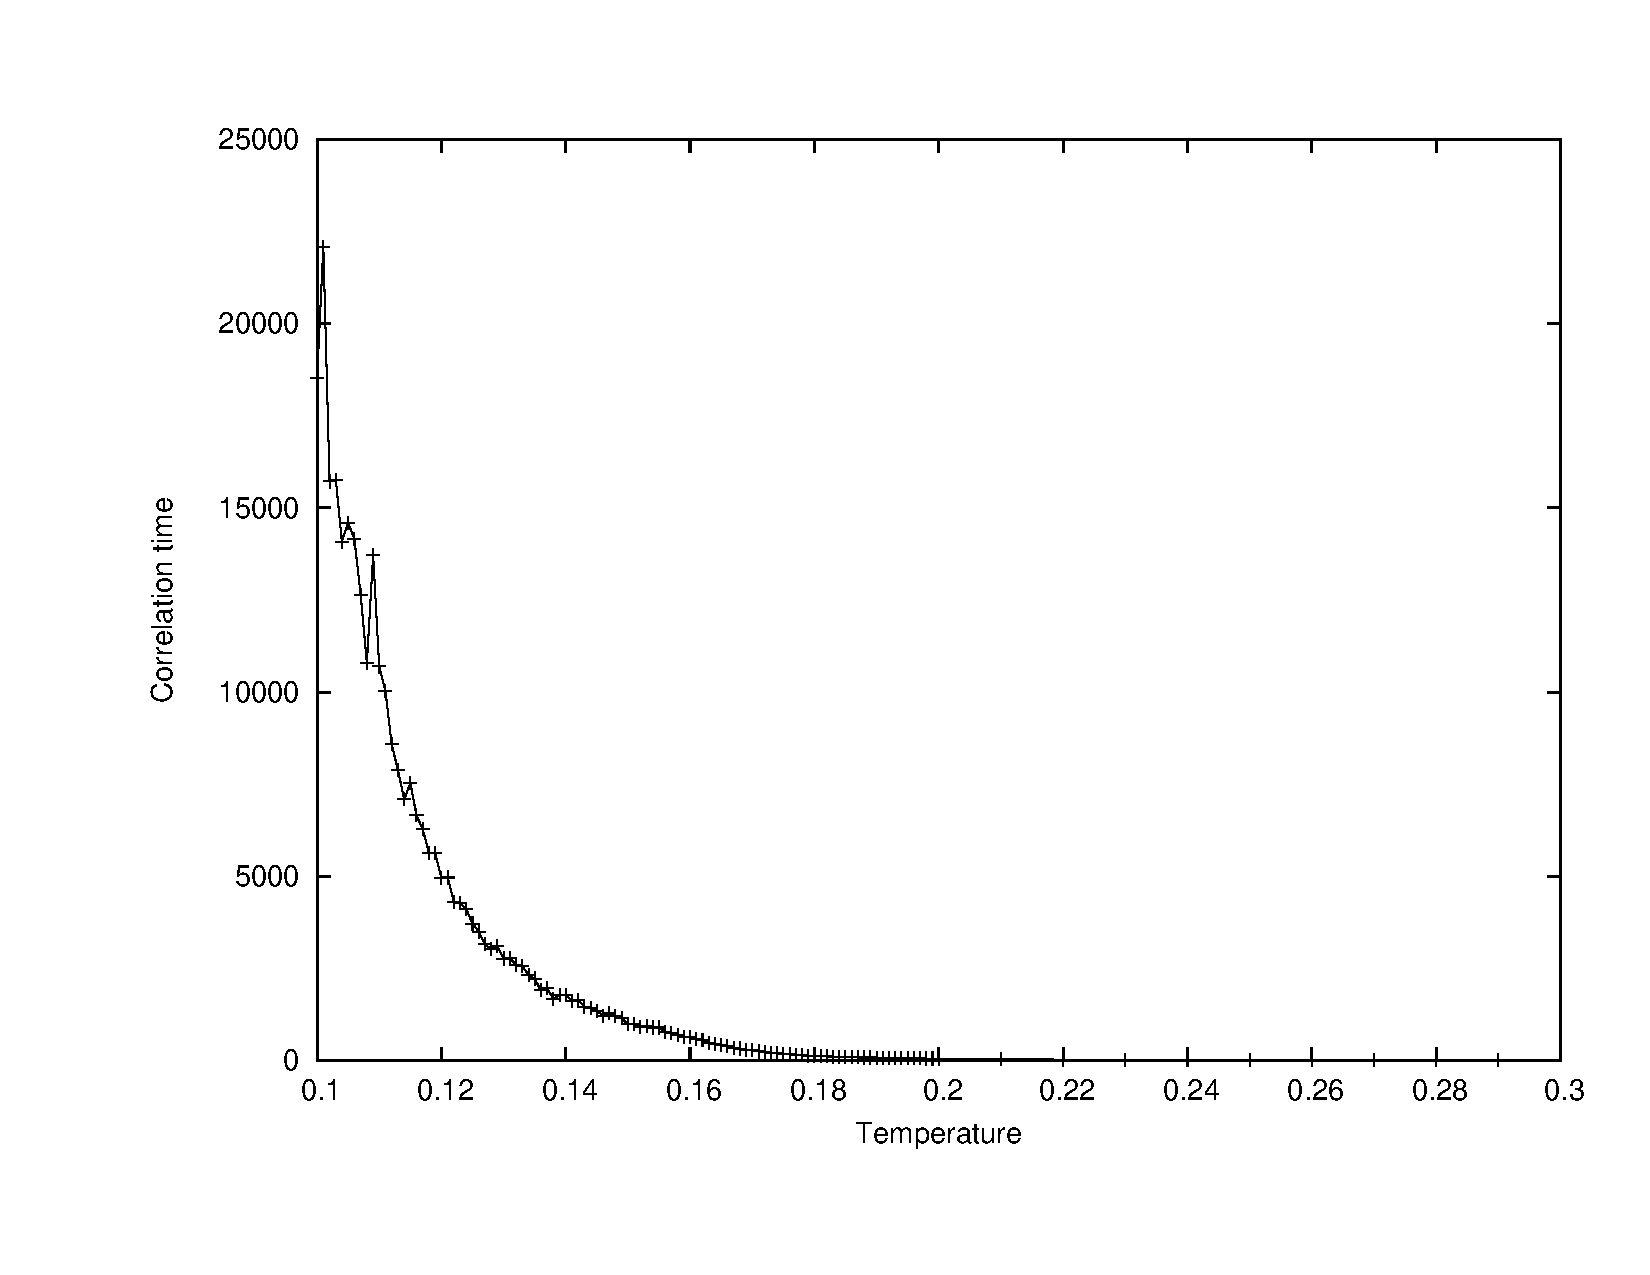
\includegraphics[width=0.5\textwidth, clip, trim = 1.7cm 1.5cm 1cm 1cm]{images/ctimes2}
	\caption{{\footnotesize Gráfico de $\tau(T')$ para o modelo de agregação a 3D, onde T' é a temperatura reduzida ($T'\equiv\frac{k_b T}{J}$), para $\rho = 0.2$, com os pontos experimentais ligados por uma linha. A estimativa do tempo foi obtida após equilibrar o sistema com 500000 MCS (passos de monte carlo), calculando a função de autocorrelação (eq.7) e integrando-a, assumindo a forma exponencial já referida.}}
	\label{fig:14}
\end{figurehere}

\begin{figurehere}
	\centering
		\includegraphics[width=0.5\textwidth, clip, trim = 1.7cm 1.5cm 1cm 1cm]{images/0.2/c}
	\caption{{\footnotesize Calor específico $c$ para $\rho = 0.2$, calculado após equilibrar o sistema esperando 500000 MCS e fazendo 20 medições da energia a cada 2 tempos de correlação, calculando então as suas flutuações.}}
	\label{fig:15}
\end{figurehere}

\begin{figurehere}
	\centering
		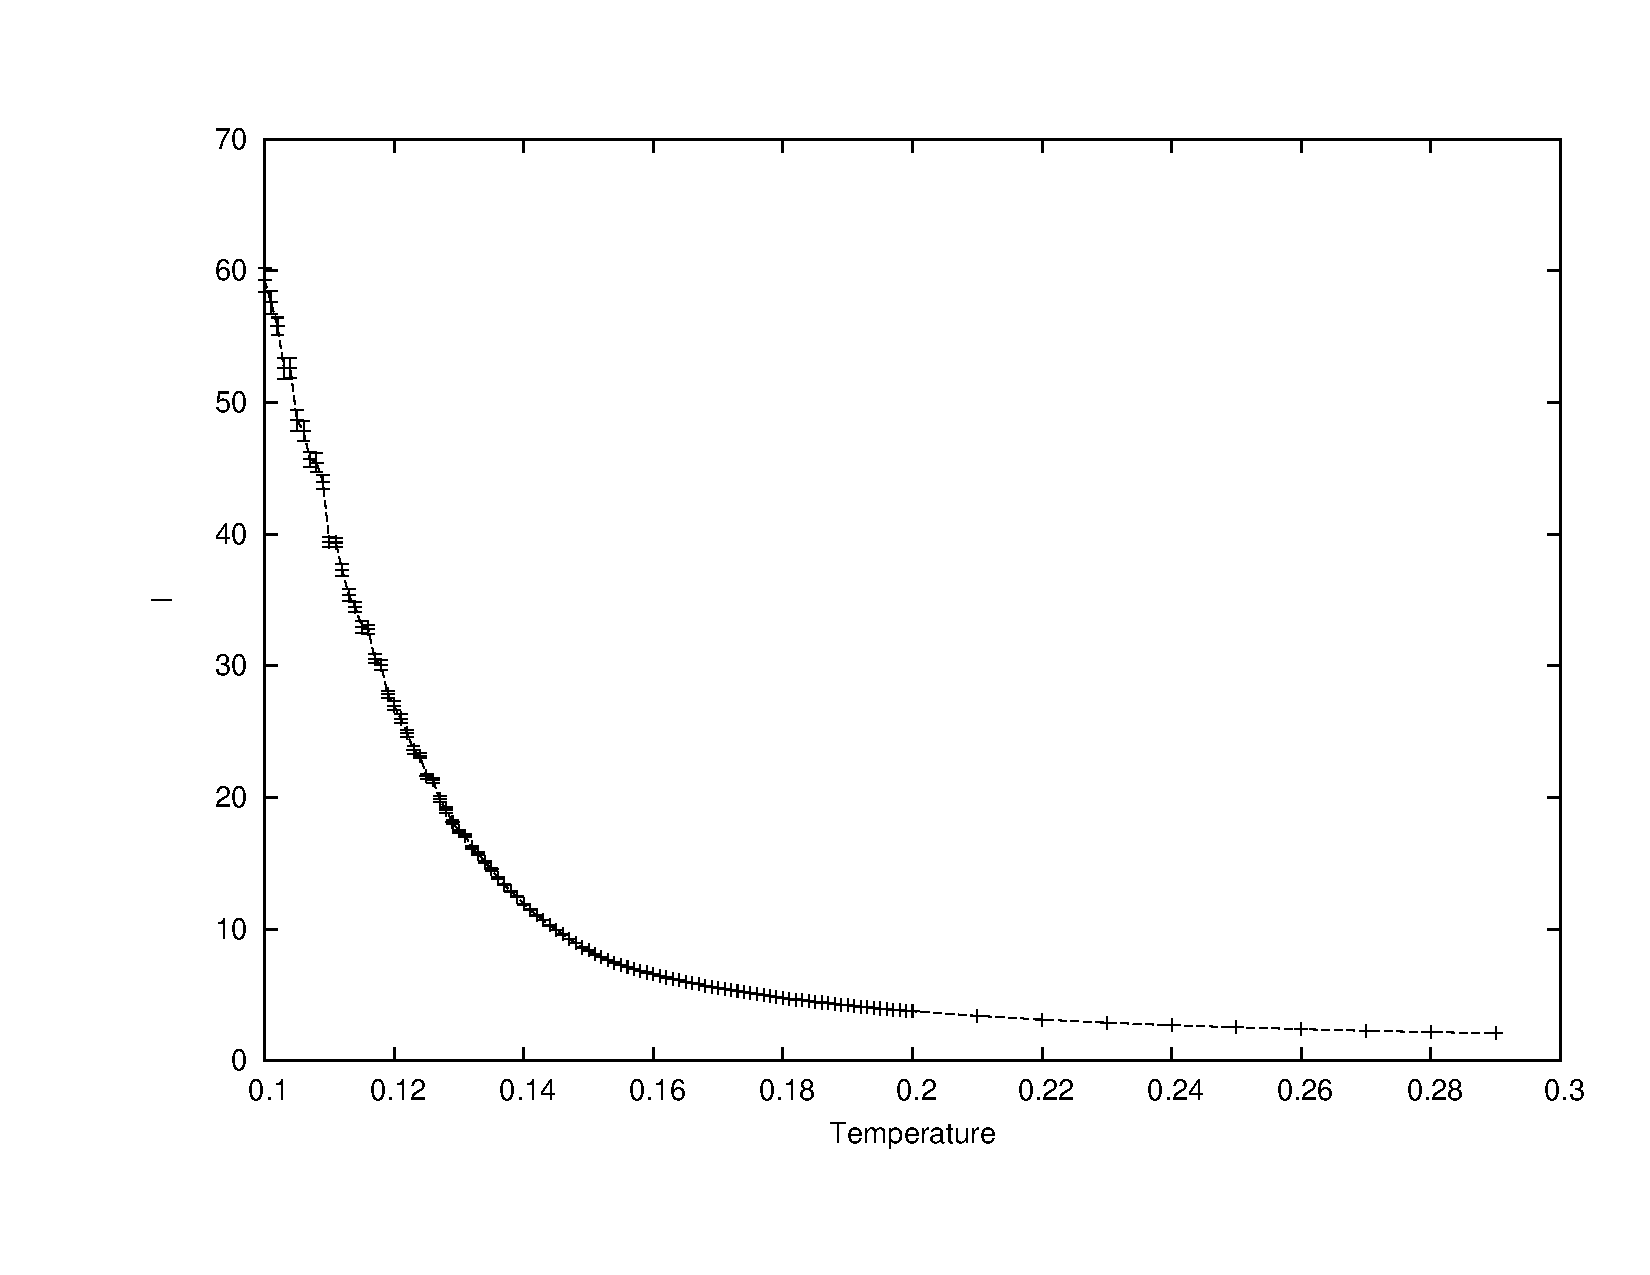
\includegraphics[width=0.5\textwidth, clip, trim = 1.7cm 1.5cm 1cm 1cm]{images/0.2/l}
	\caption{{\footnotesize Comprimento médio das cadeias $\bar{l}$ para $\rho = 0.2$, calculado após equilibrar o sistema esperando 500000 MCS e fazendo 20 medições de $\bar{l}$ a cada 2 tempos de correlação, calculando então a sua média.}}
	\label{fig:16}
\end{figurehere}

\begin{figurehere}
	\centering
		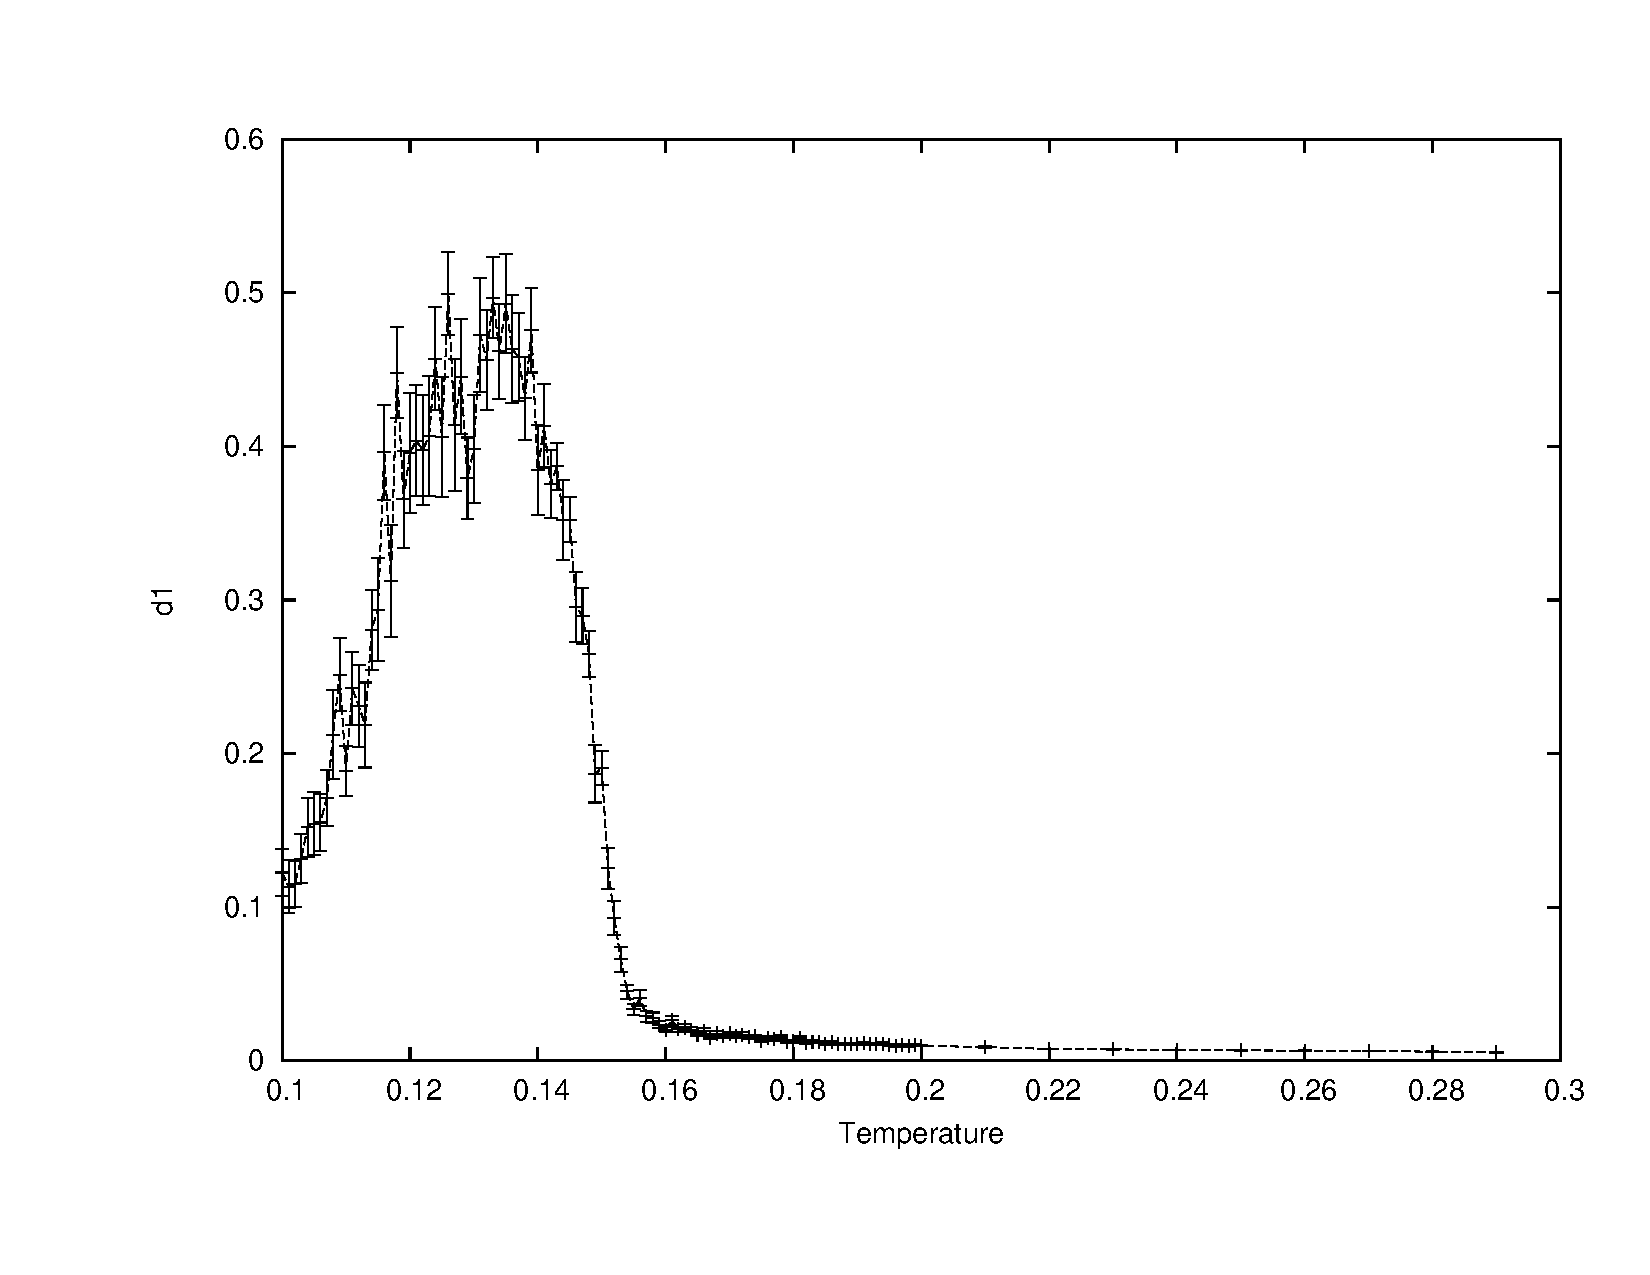
\includegraphics[width=0.5\textwidth, clip, trim = 1.7cm 1.5cm 1cm 1cm]{images/0.2/d1}
	\caption{{\footnotesize Parâmetro de ordem reduzido $|\Delta_1|$ para $\rho = 0.2$. O parâmetro foi calculado após equilibrar o sistema esperando 500000 MCS e fazendo 20 medições de $|\Delta_1|$ a cada 2 tempos de correlação, calculando então a sua média.}}
	\label{fig:17}
\end{figurehere}

\begin{figurehere}
	\centering
		\includegraphics[width=0.5\textwidth, clip, trim = 1.7cm 1.5cm 1cm 1cm]{images/0.2/d1f}
	\caption{{\footnotesize Flutuações do parâmetro de ordem reduzido $|\Delta_1|$ para $\rho = 0.2$, calculadas da mesma forma que c. Será em princípio possível ver a transição de fase determinando $T$ para a qual as flutuações tendem para infinito}}
	\label{fig:18}
\end{figurehere}

\begin{figurehere}
	\centering
		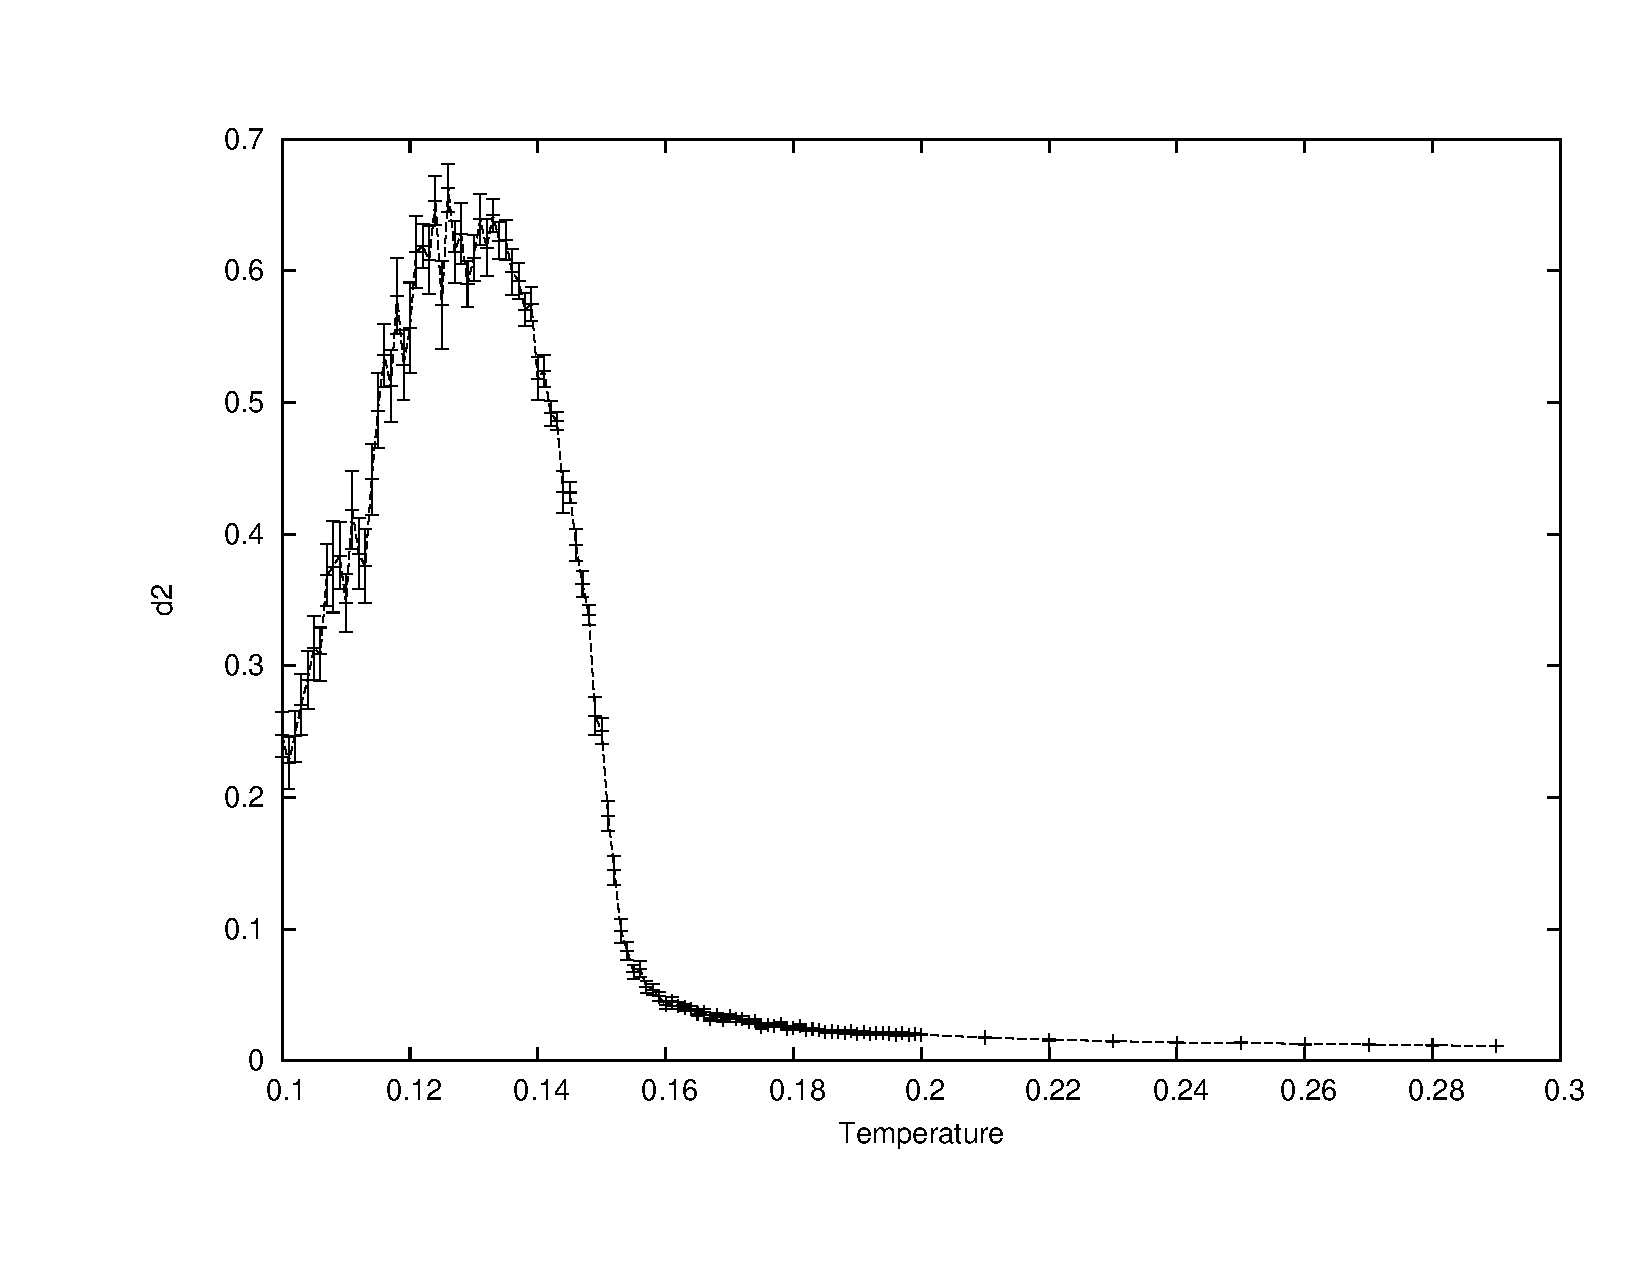
\includegraphics[width=0.5\textwidth, clip, trim = 1.7cm 1.5cm 1cm 1cm]{images/0.2/d2}
	\caption{{\footnotesize Parâmetro de ordem reduzido $|\Delta_2|$ para $\rho = 0.2$. O parâmetro foi calculado após equilibrar o sistema esperando 500000 MCS e fazendo 20 medições de $|\Delta_2|$ a cada 2 tempos de correlação, calculando então a sua média.}}
	\label{fig:19}
\end{figurehere}

\begin{figurehere}
	\centering
		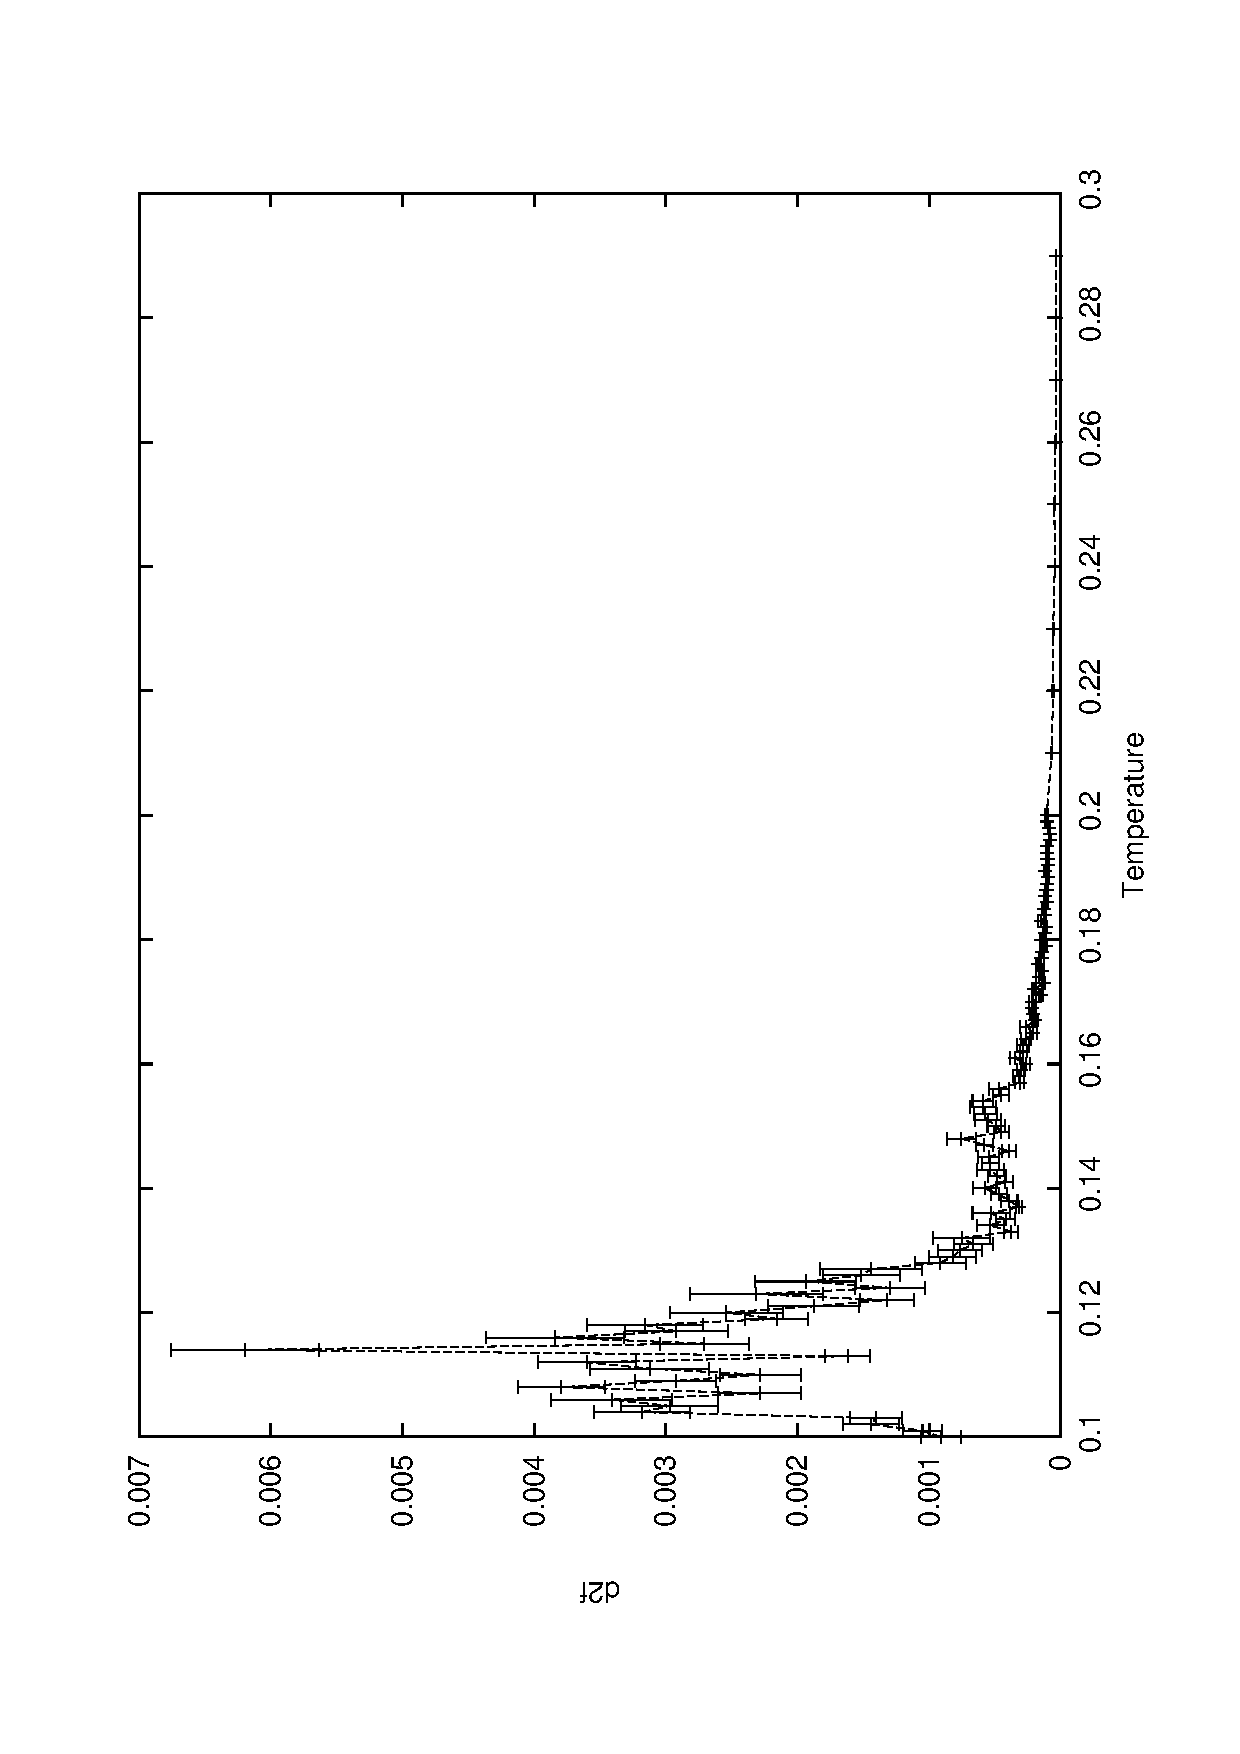
\includegraphics[width=0.5\textwidth, clip, trim = 1.7cm 1.5cm 1cm 1cm]{images/0.2/d2f}
	\caption{{\footnotesize Flutuações do parâmetro de ordem reduzido $|\Delta_2|$ para $\rho = 0.2$, calculadas da mesma forma que c. Será em princípio possível ver a transição de fase determinando $T$ para a qual as flutuações tendem para infinito}}
	\label{fig:20}
\end{figurehere}

\subsubsection{Visualização}

\begin{figurehere}
	\centering
		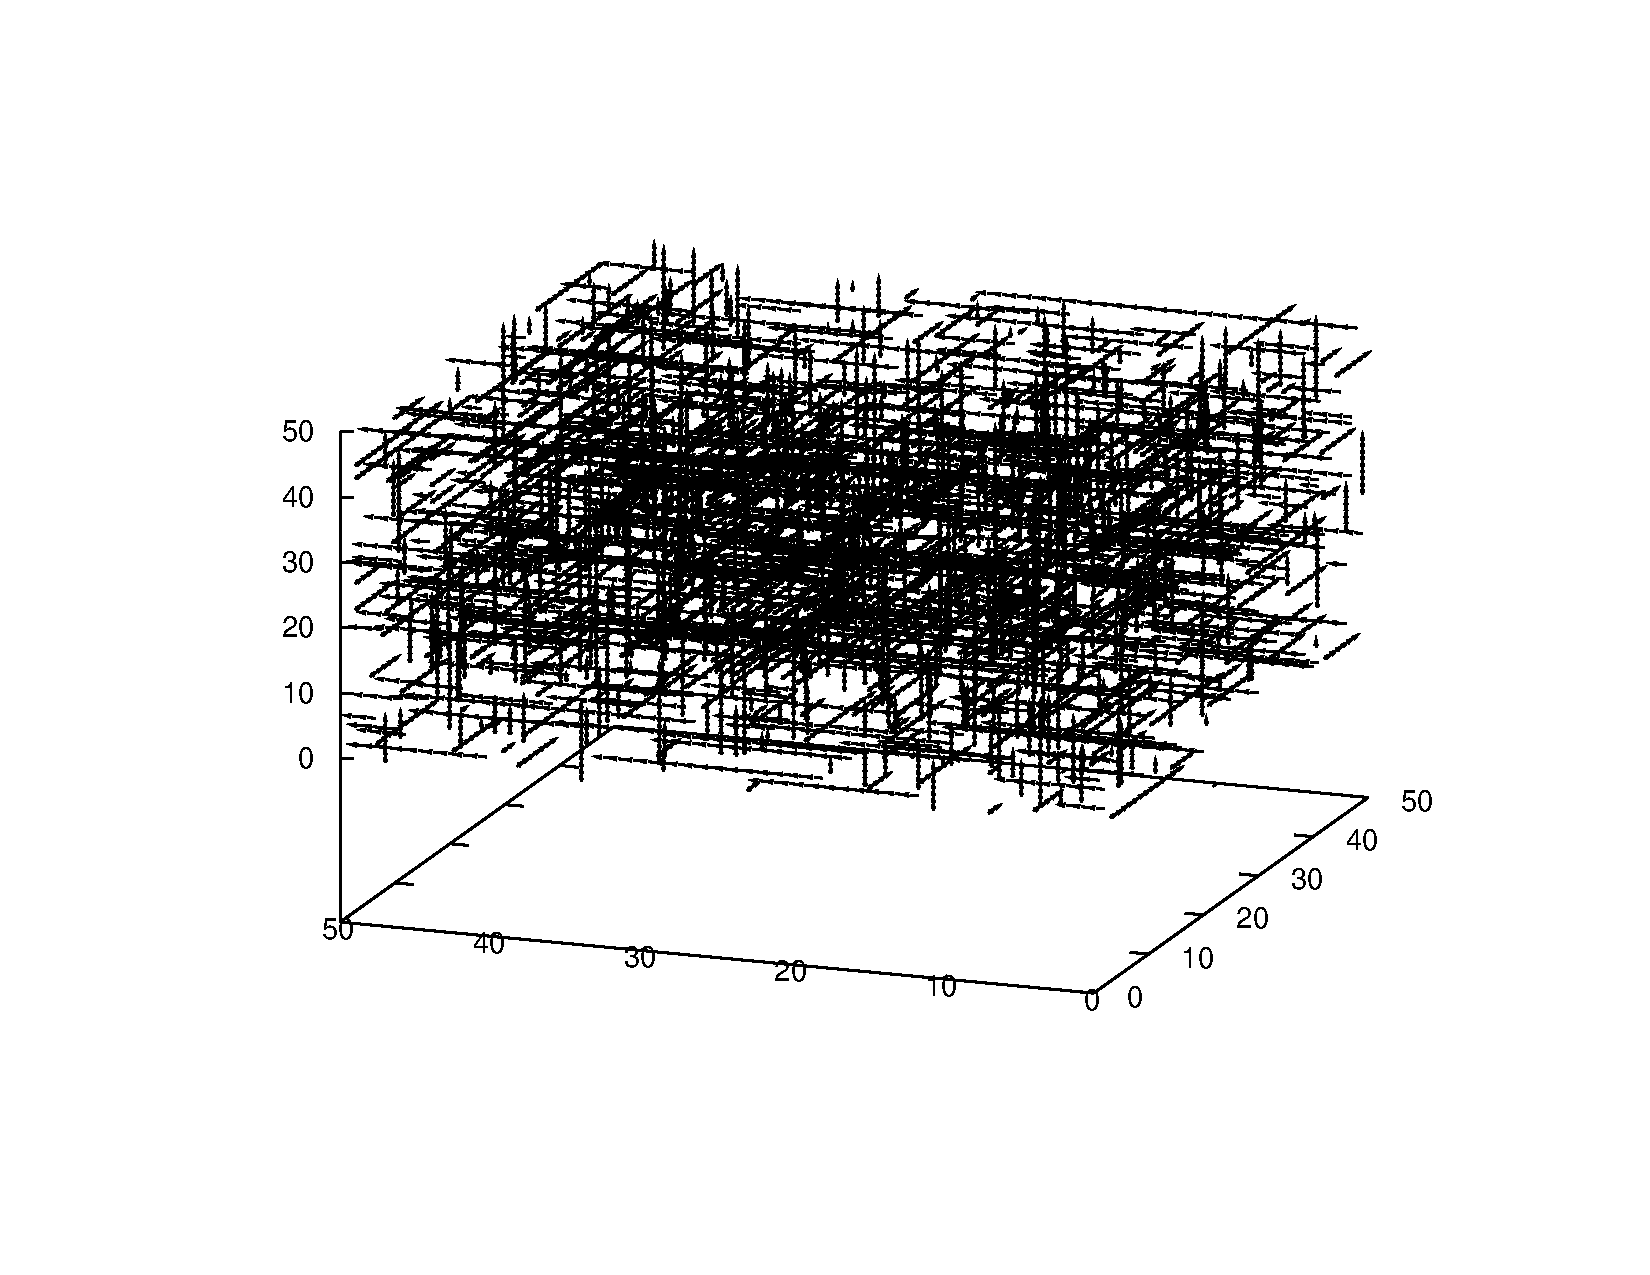
\includegraphics[width=0.5\textwidth, clip, trim = 2.7cm 2.5cm 2cm 2cm]{images/rods3d}
	\caption{{\footnotesize Visualização do sistema 3D numa rede com L=50 para $T=0.1$, onde as partículas são representadas por vectores orientados pela respectiva direcção. Visualização criada a partir de uma configuração de um sistema equilibrado após 500000 MCS. Apesar da dificuldade de visualização a 3D, para esta densidade pequena é visivel a orientação das partículas em planos, e torna-se óbvio que a dimensão acrescida remove o constrangimento de crescimento para as orientações não predominantes.}}     
	\label{fig:21}
\end{figurehere}

\bibliographystyle{plain}
\bibliography{thebib}

\end{multicols}
\end{document}